\documentclass{article} % For LaTeX2e
% ICLR 2027 submission version. Authors are hidden automatically while
% \iclrfinalcopy (below) stays commented out: the style file prints
% "Anonymous authors / Paper under double-blind review" in place of \author.
\usepackage{iclr2027_conference,times}

\usepackage[utf8]{inputenc} % allow utf-8 input
\usepackage[T1]{fontenc}    % use 8-bit T1 fonts
\usepackage{hyperref}       % hyperlinks
\usepackage{url}            % simple URL typesetting
\usepackage{booktabs}       % professional-quality tables
\usepackage{amsfonts}       % blackboard math symbols
\usepackage{nicefrac}       % compact symbols for 1/2, etc.
\usepackage{microtype}      % microtypography
\usepackage{xcolor}
\usepackage{multirow}
\usepackage{enumitem}
\usepackage{amsmath,amssymb,amsthm}
\usepackage{graphicx}
\usepackage{wrapfig}
\usepackage{subcaption}
\usepackage{array}
\usepackage{tabularx}
\usepackage{placeins}

\newcolumntype{Y}{>{\raggedright\arraybackslash}X}

%%%%%%%%%%%%%%%%%%%%%%%%%%%%%%%%
% THEOREMS
%%%%%%%%%%%%%%%%%%%%%%%%%%%%%%%%
\theoremstyle{plain}
\newtheorem{theorem}{Theorem}[section]
\newtheorem{proposition}[theorem]{Proposition}
\newtheorem{lemma}[theorem]{Lemma}
\newtheorem{corollary}[theorem]{Corollary}
\theoremstyle{definition}
\newtheorem{definition}[theorem]{Definition}
\newtheorem{assumption}[theorem]{Assumption}
\theoremstyle{remark}
\newtheorem{remark}[theorem]{Remark}
\theoremstyle{problem}
\newtheorem{problem}[theorem]{Problem}

\title{ReAD: Reinforcement-Guided Capability Distillation for Large Language Models}

% Author names and affiliations were removed from this source for the
% double-blind submission. Fill them in (see iclr2027_conference.tex for the
% \author / \And / \AND format) and uncomment \iclrfinalcopy for camera-ready.
\author{Anonymous authors}

\newcommand{\xq}[1]{{\color{red}{#1}}}
% Revision markup: text added or changed in the ICLR revision is shown in red.
% Before submission, switch it off with:  \renewcommand{\rev}[1]{#1}
\newcommand{\rev}[1]{#1}  % revision markup kept in the source; set to {{\color{red}{}#1}} to show changes in red
% keep a heading with the lines that follow it (same idea as needspace.sty)
\makeatletter
\newcommand{\keepwithnext}[1]{\par\vskip\z@\@plus#1\penalty-100\vskip\z@\@plus-#1}
\makeatother

%\iclrfinalcopy % Uncomment for camera-ready version, but NOT for submission.
\begin{document}

\maketitle

% ============================================================
\begin{abstract}
\rev{Capability distillation specializes a smaller language model toward a specified capability using supervision from a larger teacher. Under a fixed distillation-token budget, an important question is how to allocate supervision across capabilities to improve the target most effectively. Our empirical study shows that single-capability distillation produces budget-dependent cross-capability changes and diminishing target gains, motivating allocation strategies that adapt to the student's evolving state. We propose \textit{ReAD}, a \textit{Re}inforcement-guided c\textit{A}pability \textit{D}istillation framework that combines a task-conditioned allocation prior, on-the-fly teacher supervision, and an uncertainty-aware contextual bandit. ReAD updates its allocation using measured capability changes, rewarding task-aligned gains and penalizing regressions on prioritized capabilities. Across eight target capabilities, two teacher--student pairs, and two token budgets, ReAD achieves higher mean on-target scores than the evaluated target-only baselines. Matched-generator comparisons show additional gains over static and greedy allocation schedules, while transfer diagnostics show smaller off-target declines.} Our code is available at
\url{https://anonymous.4open.science/r/ReAD-62B7}. % camera-ready: replace with the public repository link
\end{abstract}

\section{Introduction}
\label{sec:intro}

Knowledge distillation (KD)~\citep{hinton2015distilling} for large language models (LLMs)~\citep{zhao2023survey} has become an essential research direction for enhancing the accessibility and efficiency of Machine-Learning-as-a-Service (MLaaS)~\citep{cai2024llmaas,xu2024survey_kd_llms,yang2024survey_kdllm}. Through knowledge distillation, a small LLM learns to imitate a large teacher LLM's outputs, enabling effective deployment under limited computational or financial resources~\citep{sanh2019distilbert,jiao2020tinybert,wang2020minilm,li2021dynamickd,liang2023less}. Recent studies show that capability distillation, a specialization of knowledge distillation that focuses supervision on a target capability (e.g., instruction-following, reasoning, mathematics, or coding), can substantially improve the student’s performance on downstream tasks that primarily depend on that capability, while achieving these gains at lower serving cost than the large teacher model~\citep{magister2023teaching,shridhar2022distilling,xu2023wizardlm,yue2024distilling}.
% \yd{we seem to mix learning capabilities and knowledge distillation here. They are not interchangable. Let's make their relationship clearer: knowledge distillation does not equal to learning capabilities; learning capabilities is a type of the broader definition of KD.}


Despite rapid progress in capability distillation, most existing methods still treat capabilities as if they can be improved independently~\citep{taori2023stanford, chiang2023vicuna,zhang2024knowledgeable}, even though empirical evidence suggests that optimizing one capability often triggers broad, unintended shifts in the model’s overall capability profile~\cite {zhong2024revisiting, fang2025kddd_survey,cloud2025subliminal}. This mismatch is especially consequential in the budgeted setting: under a fixed token budget, the goal is to maximize downstream task utility, which depends not only on the targeted capability but also on other capabilities the task may implicitly require. If cross-capability interactions are ignored, allocating more tokens to a single target can become inefficient in two ways: the extra improvement on the target can shrink as the budget grows, and the same updates may reduce performance on other tasks that require non-target capabilities. In this case, additional tokens are effectively spent on updates that provide little task-relevant benefit and may even increase deployment risk in MLaaS, which we refer to as \emph{budget waste}. To systematically examine this gap, we take a first step toward measuring and understanding these interactions through a controlled empirical study. Concretely, we repeatedly distill the student under multiple token budgets, each time allocating the entire budget to one target capability drawn from a set of widely recognized core LLM capabilities: General Knowledge (General), Reasoning, Math, Code, Tool use, Long-Context Understanding (LCU), Steerability, and Multilinguality. After each run, we evaluate the resulting student on the full benchmark suite in Table~\ref{tab:capabilities-benchmarks} and record the score change for every capability. This yields a budget-dependent capability transfer matrix in which the diagonal entries capture on-target improvement and the off-diagonal entries capture how training toward one capability redistributes performance across the others. Across budgets, we observe two consistent patterns: \textit{(i) capability-specific distillation induces systematic, budget-dependent transfer to other capabilities rather than isolated improvements}, and \textit{(ii) increasing the budget for a single target produces smaller additional target gains while making the average harm to non-target capabilities more pronounced}, which together explain why naively scaling the budget for one capability can be inefficient.
% \yd{I think you have not clarify any goal yet. what are people trying achieve? you mean the challenges of trying to achieve what? trying to distill one capability without changing the level of other capabilities? or use the least budget to achieve the best distillation for one capability regardless of other capabilities?} 
% First, improving one target capability frequently causes noticeable shifts in other latent capabilities; second, many of the capabilities enhanced during distillation provide little or no benefit to the downstream task, which means that a portion of the optimization budget is spent on capabilities with low task utility. Without understanding these challenges, capability distillation can misallocate training budgets, alter unrelated capabilities, and produce unpredictable behaviors, posing higher cost and safety concerns for MLaaS deployment.

% In this paper, we take a first step toward understanding capability distillation from a more fundamental perspective. Specifically, capability distillation can be interpreted as compressing a large model into a smaller one that retains only the capabilities needed for a target task, making the student a compact representation of the teacher’s task-relevant intelligence. Since classical theories view intelligence as arising from compression \yd{how this claim connects to your story reads vague and suspicious. intelligence cannot arise from any type of compression over anything. Then is this the type of compression your story is referring to?}, where effective behavior is produced by forming compact representations that support prediction and decision-making~\citep{solomonoff1964formal, wallace1999minimum,hutter2000theory}, this perspective suggests that an LLM’s intelligence can be understood as a composition of interacting capabilities that jointly determine its competence. From this viewpoint, two questions naturally follow: \textit{(1) What is the empirical structure of compressed intelligence when expressed through capabilities}, and \textit{(2) How %%\td{consistency with What/what and How/how}
% %how 
% should a limited distillation budget be allocated to acquire the capabilities required for a specific task?} \yd{the two questions are vague. 1 - What can be an empirical structure of compressed intelligence? a star or a triangle? Audience does not know what specifically you are referring to. 2 - budget allocated over what? you already targeted on a capability so we are still allocating budget on other capabilities (if so why? why do not we directly allocate all on the targeted capability?)? or on other data points?} To answer these questions, we conduct extensive experiments to show that: \textit{(i) capability distillation induces systematic, budget-dependent cross-capability transfer}, and \textit{(ii) capability distillation suffers from diminishing returns and negative spillover, leading to substantial budget waste} 
% \yd{still, using private names without definition or explanation wipes out the meaning of this claim.}.\xq{explain in here and in obs 2}

Building on these observed insights, we propose \textit{ReAD}, a \textit{Re}inforcement-guided c\textit{A}pability \textit{D}istillation framework for large language models. Overall, ReAD combines on-the-fly capability-targeted data generation with token-level knowledge distillation, and uses a lightweight contextual bandit to adaptively allocate a fixed budget across interdependent capabilities. Specifically, ReAD first infers a task requirement vector that identifies which capabilities are essential for improving the downstream utility and treats degradations on these dimensions as harmful spillover. It then allocates distillation effort to maximize a proxy reward that favors capability gains aligned with the task requirements while penalizing spillover and budget consumption. In each interval, ReAD samples capability-labeled prompts according to the current allocation, queries the teacher to obtain supervision, updates the student with a standard distillation loss, and uses the resulting capability-profile change to update an uncertainty-aware UCB allocation rule. Extensive experiments demonstrate that ReAD strengthens task-relevant capabilities and reduces wasted budget on low-utility capability updates under budget constraints.

To sum up, this paper makes the following key contributions: 
% \yd{names are not parallel - they do not match each other on the same level. Also, let's make the description more balanced.}

\begin{itemize}[leftmargin=*, itemsep=1pt, topsep=1pt]
    \item \textbf{Empirical study of cross-capability interactions.}
    We show that distilling toward a single capability consistently changes other capabilities, revealing systematic cross-capability interactions that are often overlooked.
    
    \item \textbf{Budgeted capability distillation formulation.}
    We formulate capability distillation as allocating a fixed budget across multiple interacting capabilities, providing objective for improving utility while controlling side effects.
    
    \item \textbf{ReAD: reinforcement-guided capability distillation.}
    ReAD infers task-relevant capabilities, generates capability-targeted distillation data with controllable style and difficulty, and uses an uncertainty-aware contextual bandit to allocate the budget across capabilities.
    
    \item \textbf{Theory analysis of the capability interdependence.}
    We explain cross-capability interactions and diminishing returns in capability distillation.
\end{itemize}
\section{Preliminary}
\label{sec:prelim}

\subsection{Notation and Formalization}

In this paper, we study budgeted capability distillation from a large teacher model \(T\) to a
smaller student model \(S\), with total training-token budget \(B\). Let
\(\mathcal{C}=\{c_1,\ldots,c_{|\mathcal{C}|}\}\) denote a set of measurable
capabilities\rev{, here the eight core capabilities of Appendix Table~\ref{tab:capabilities-benchmarks},} and let \(s_k(M)\) be model \(M\)'s benchmark score on capability
\(c_k\). A distillation strategy \(\pi\) specifies how data is generated, how
the teacher is queried, and how tokens are allocated across capabilities,
assigning budgets \(\{b_k\}\) with \(\sum_k b_k\le B\), and producing a
distilled student \(S_\pi\).

\begin{definition}[Capability distillation]\label{def:cap_distill}
Given a teacher model \( T \), an initial student model \( S_0 \), and
capability-specific data distributions \( \{ \mathcal{D}_c \}_{c\in\mathcal{C}} \),
capability distillation allocates a limited budget \( B \) across capabilities
to improve task-relevant performance under shared representations by optimizing
a weighted mixture of distillation objectives:
\begin{equation}
\begin{aligned}
\min_{S,\,\mathbf{w}} \;&
\mathbb{E}_{x\sim \mathcal{D}_{\mathbf{w}}}
\!\left[\ell\!\left(S(x),T(x)\right)\right] \quad\
\text{s.t.} \quad\
\mathbf{w}\in\Delta_{|\mathcal{C}|},\; \mathrm{cost}(S;S_0)\le B .
\end{aligned}
\end{equation}
where \( \mathcal{D}_{\mathbf{w}} := \sum_{c\in\mathcal{C}} w_c \mathcal{D}_c \), and $\mathrm{cost}(S;S_0)$ measures the distillation token budget consumed to obtain $S$ from $S_0$.
Here \( \mathbf{w}=(w_c)_{c\in\mathcal{C}} \) lies in the probability simplex
\rev{\( \Delta_{|\mathcal{C}|}=\{\mathbf{w}\in\mathbb{R}^{|\mathcal{C}|} \mid w_c\ge 0,\ \sum_{c\in\mathcal{C}} w_c=1\} \)},
which specifies the allocation of training effort across capabilities, and
\( \ell \) denotes a standard distillation loss, such as token-level
cross-entropy or logit-matching between the student\rev{'s and the teacher's output distributions}.
\end{definition}

\rev{Under shared representations, budget spent on one capability changes the
others. We measure this cross-capability effect by distilling with one-hot allocations:}
\begin{definition}[Capability interdependence]\label{def:cap_interdependence}
Let \( S_0 \) be an initial student model, and let \( S(\mathbf{w},B) \) denote
the student obtained after capability distillation under allocation
\( \mathbf{w}\in\Delta_{|\mathcal{C}|} \) and budget \( B \). For each capability
\( c_i \), define the one-hot allocation vector
\( \mathbf{w}^{(i)}\in\Delta_{|\mathcal{C}|} \) by \( w^{(i)}_i=1 \) and
\( w^{(i)}_j=0 \) for all \( j\neq i \). The \emph{capability interdependence}
under capability distillation is characterized by the capability transfer matrix
\[
\mathbf{T}_{ij}(B)
:= s_j\!\left(S(\mathbf{w}^{(i)},B)\right) - s_j(S_0),
\]
where $\mathbf{T}(B)\in\mathbb{R}^{|\mathcal{C}|\times|\mathcal{C}|}$, \( \mathbf{T}_{ij}(B) \) quantifies the effect of distilling
toward capability \( c_i \) on the performance of capability \( c_j \).
Non-zero off-diagonal entries indicate interdependence between capabilities
under shared representations.
\end{definition}

\vspace{-0.6em}
\subsection{Exploratory Study and Problem Formulation}
\label{sec:emp_res}

\rev{We distill Llama-3.3-70B-Instruct into Llama-3.1-8B-Instruct under fixed
token budgets, one target capability at a time, and evaluate the student on all
benchmarks to form the transfer matrix of Definition~\ref{def:cap_interdependence}
(strategies and settings in Appendix~\ref{sec:app_em}). All
benchmark metrics are accuracies or success rates on a $0$--$100$ scale, a
capability score is the unweighted mean over its benchmarks, and every entry of
the transfer matrix is an absolute difference in these points
(Definition~\ref{def:cap_interdependence}); no further rescaling is applied
(Appendix~\ref{sec:app_em}).}

%==================== Figure 1: empirical study (top float; all four panels share one height) ====================
\begin{figure}[t]
  \centering
  \captionsetup[sub]{font=footnotesize,skip=2pt}
  % capability legend as a single row: the two rows of icon.pdf, cropped and placed side by side
  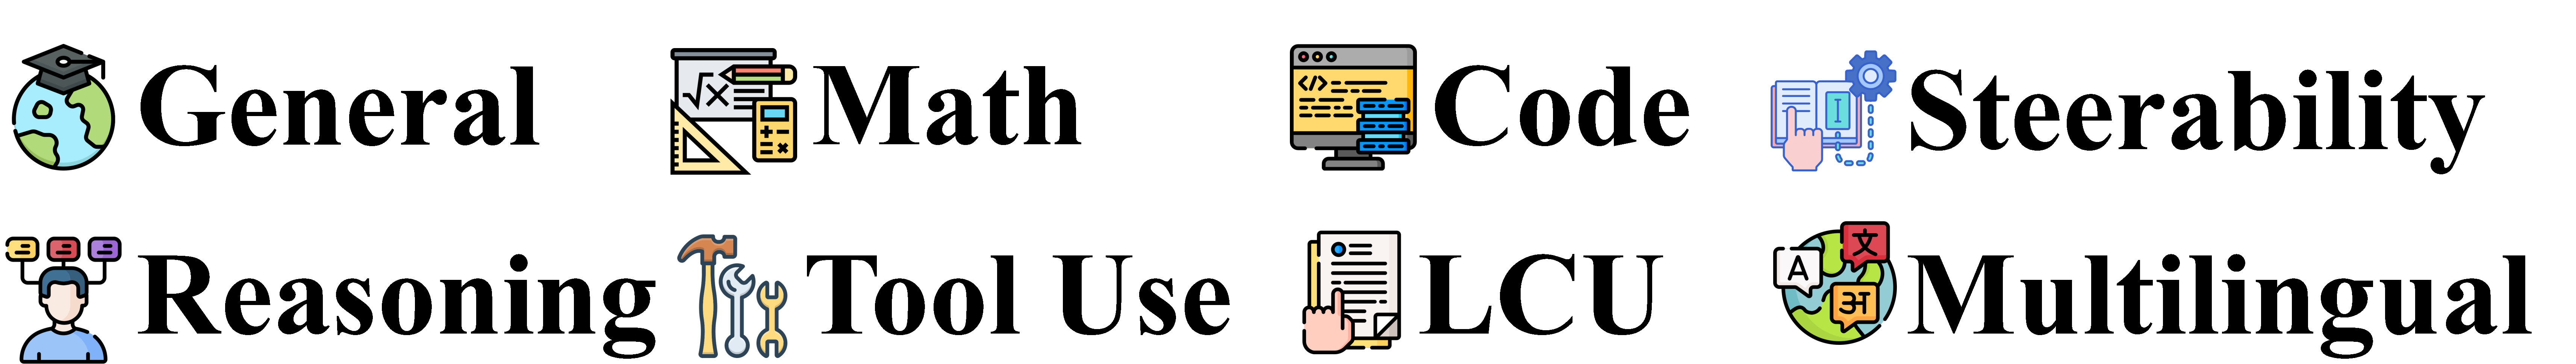
\includegraphics[height=11pt,trim=0 232 50 43,clip]{figure/icon.pdf}\hspace{0.8em}%
  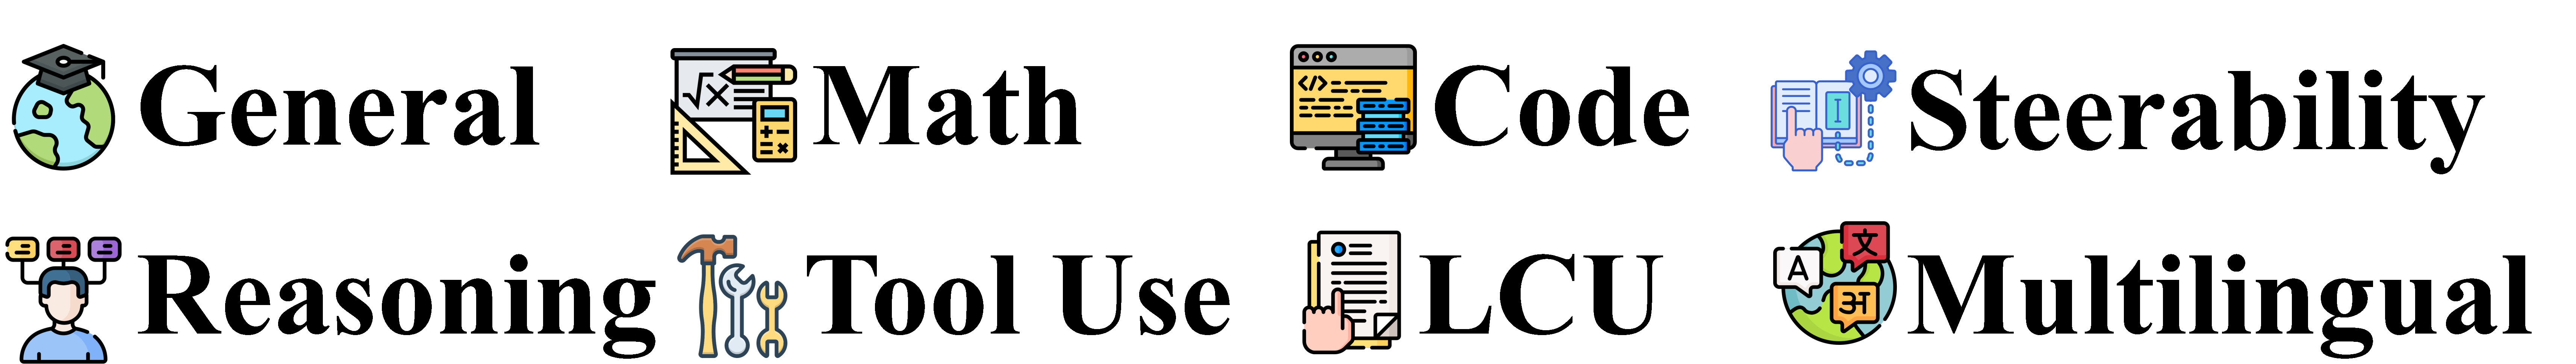
\includegraphics[height=11pt,trim=0 0 50 275,clip]{figure/icon.pdf}\\[3pt]
  % panel widths follow from a common height of 72pt and each PDF's aspect ratio
  \begin{subfigure}[b]{0.181\linewidth}
    \centering
    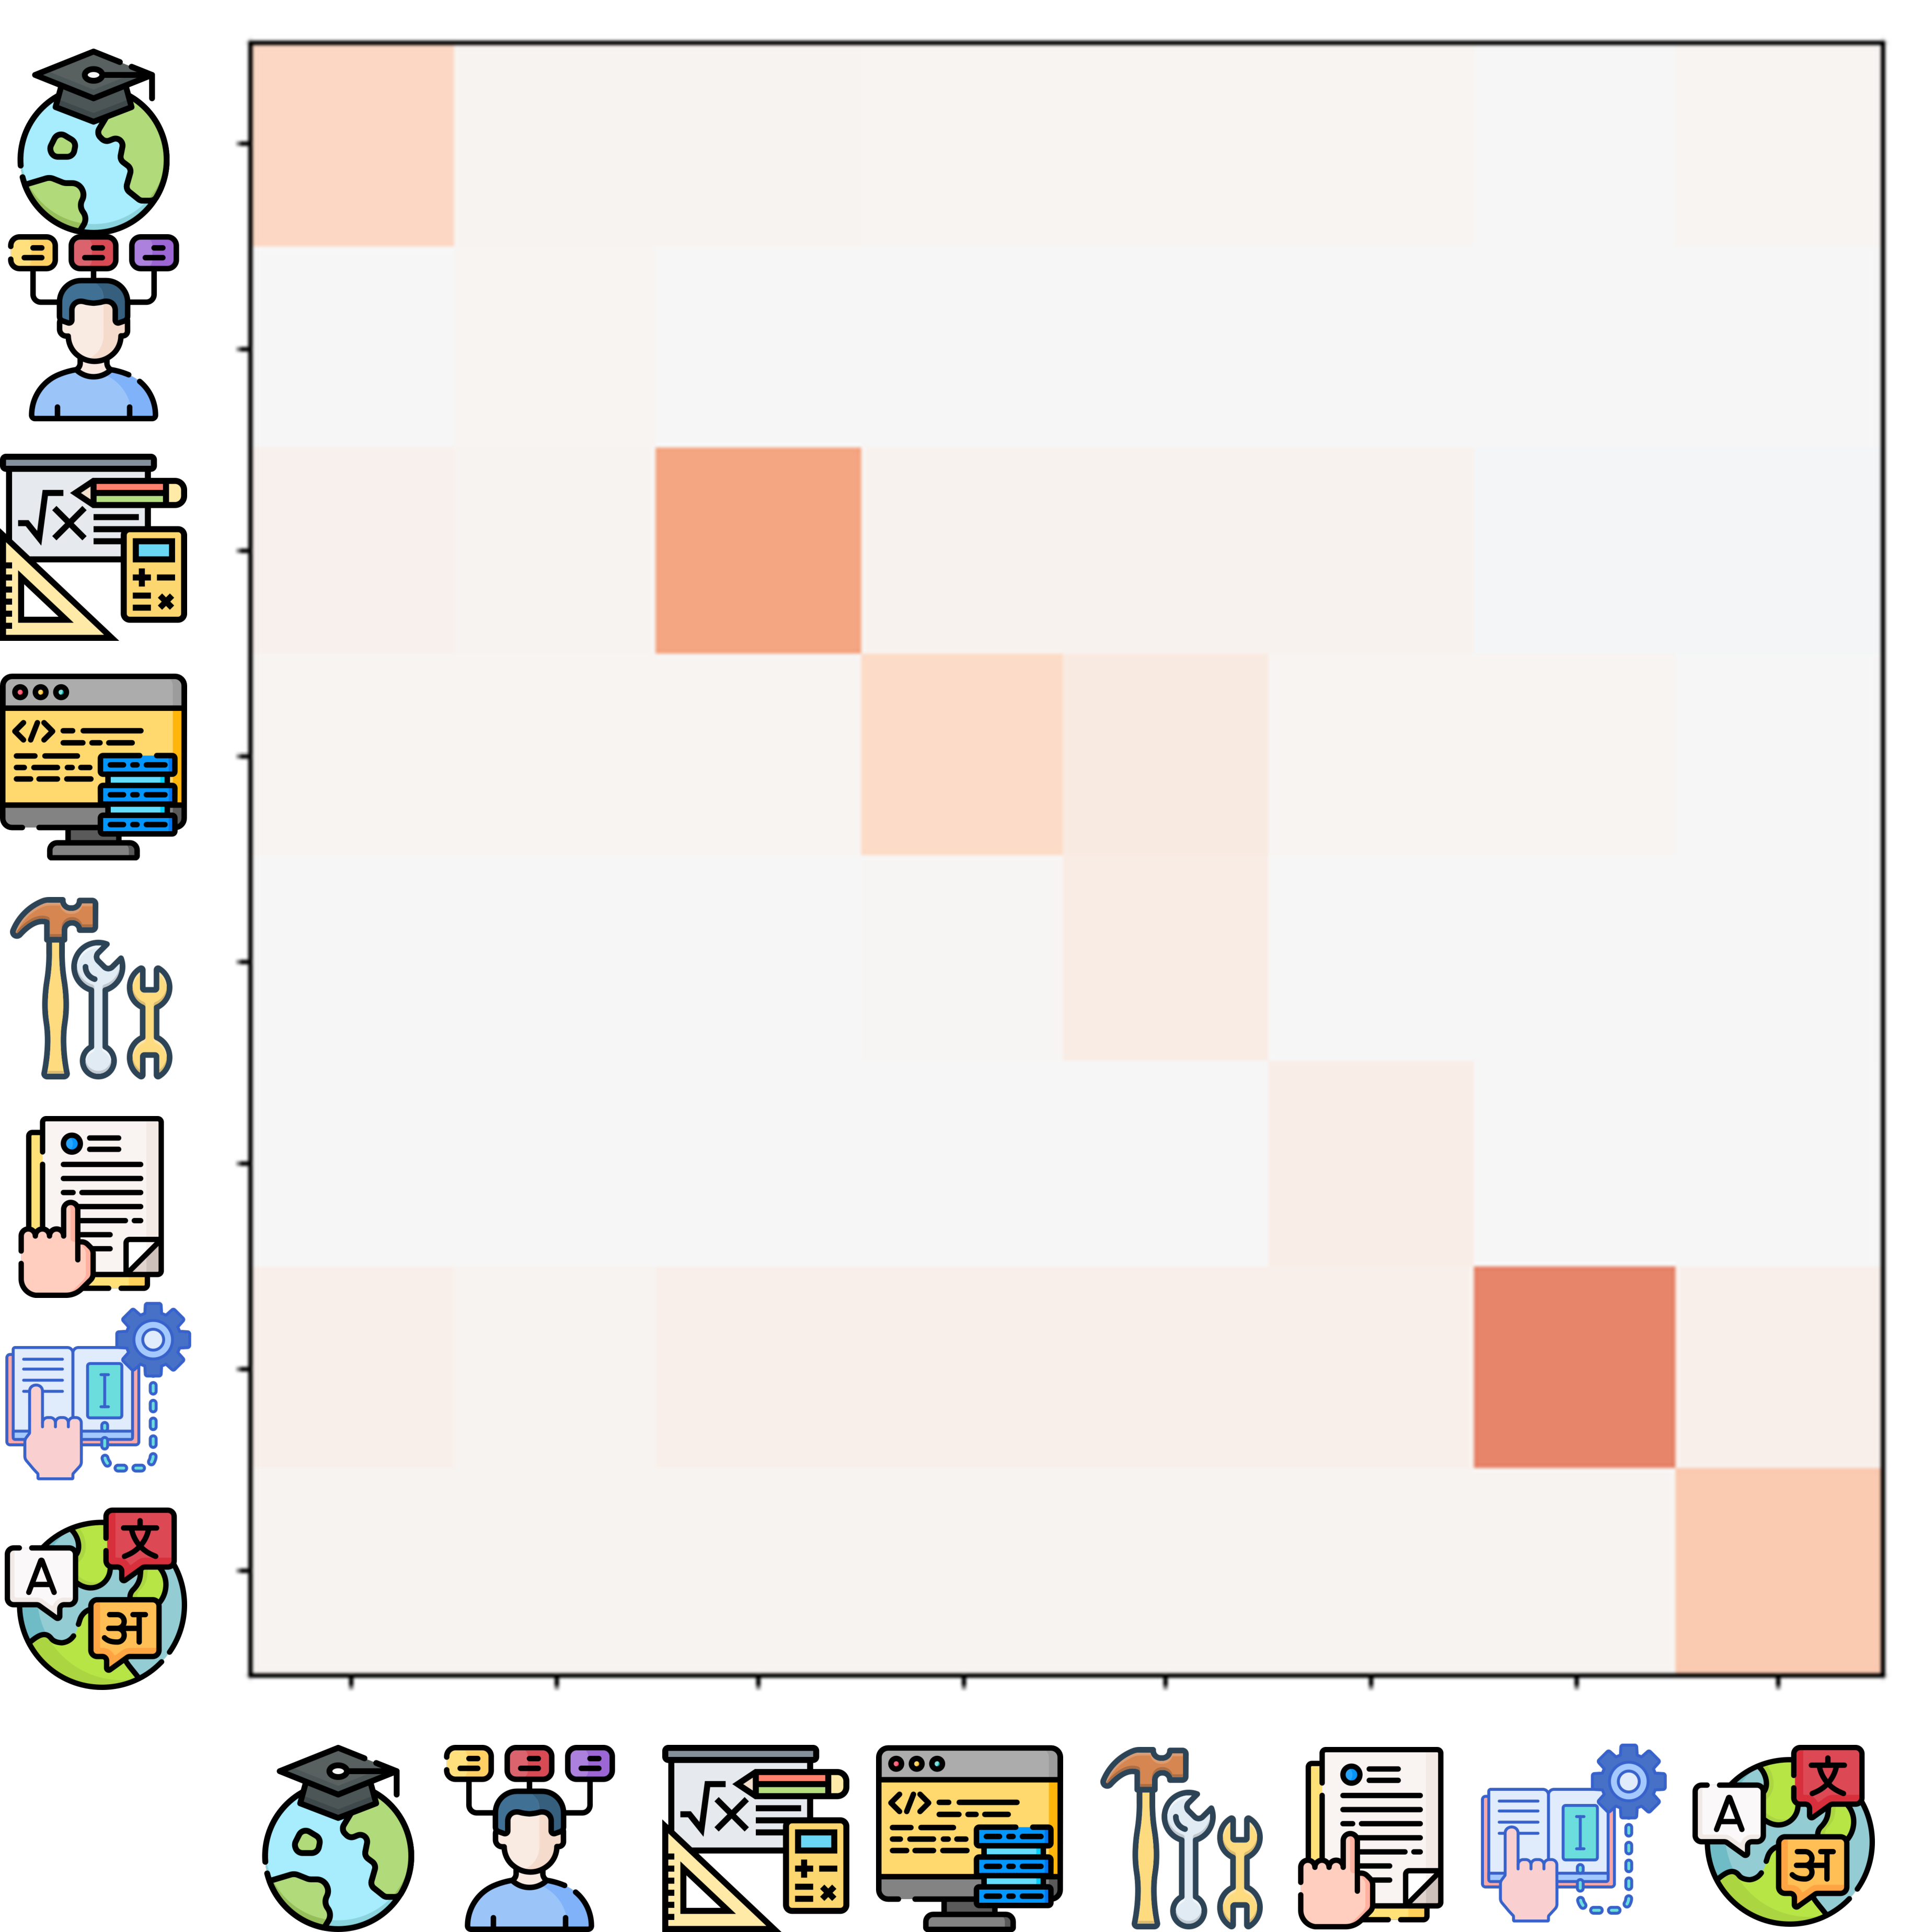
\includegraphics[height=72pt]{figure/heatmap_small.pdf}
    \caption{Small budget}
    \label{fig:heatmap_small}
  \end{subfigure}\hfill
  \begin{subfigure}[b]{0.209\linewidth}
    \centering
    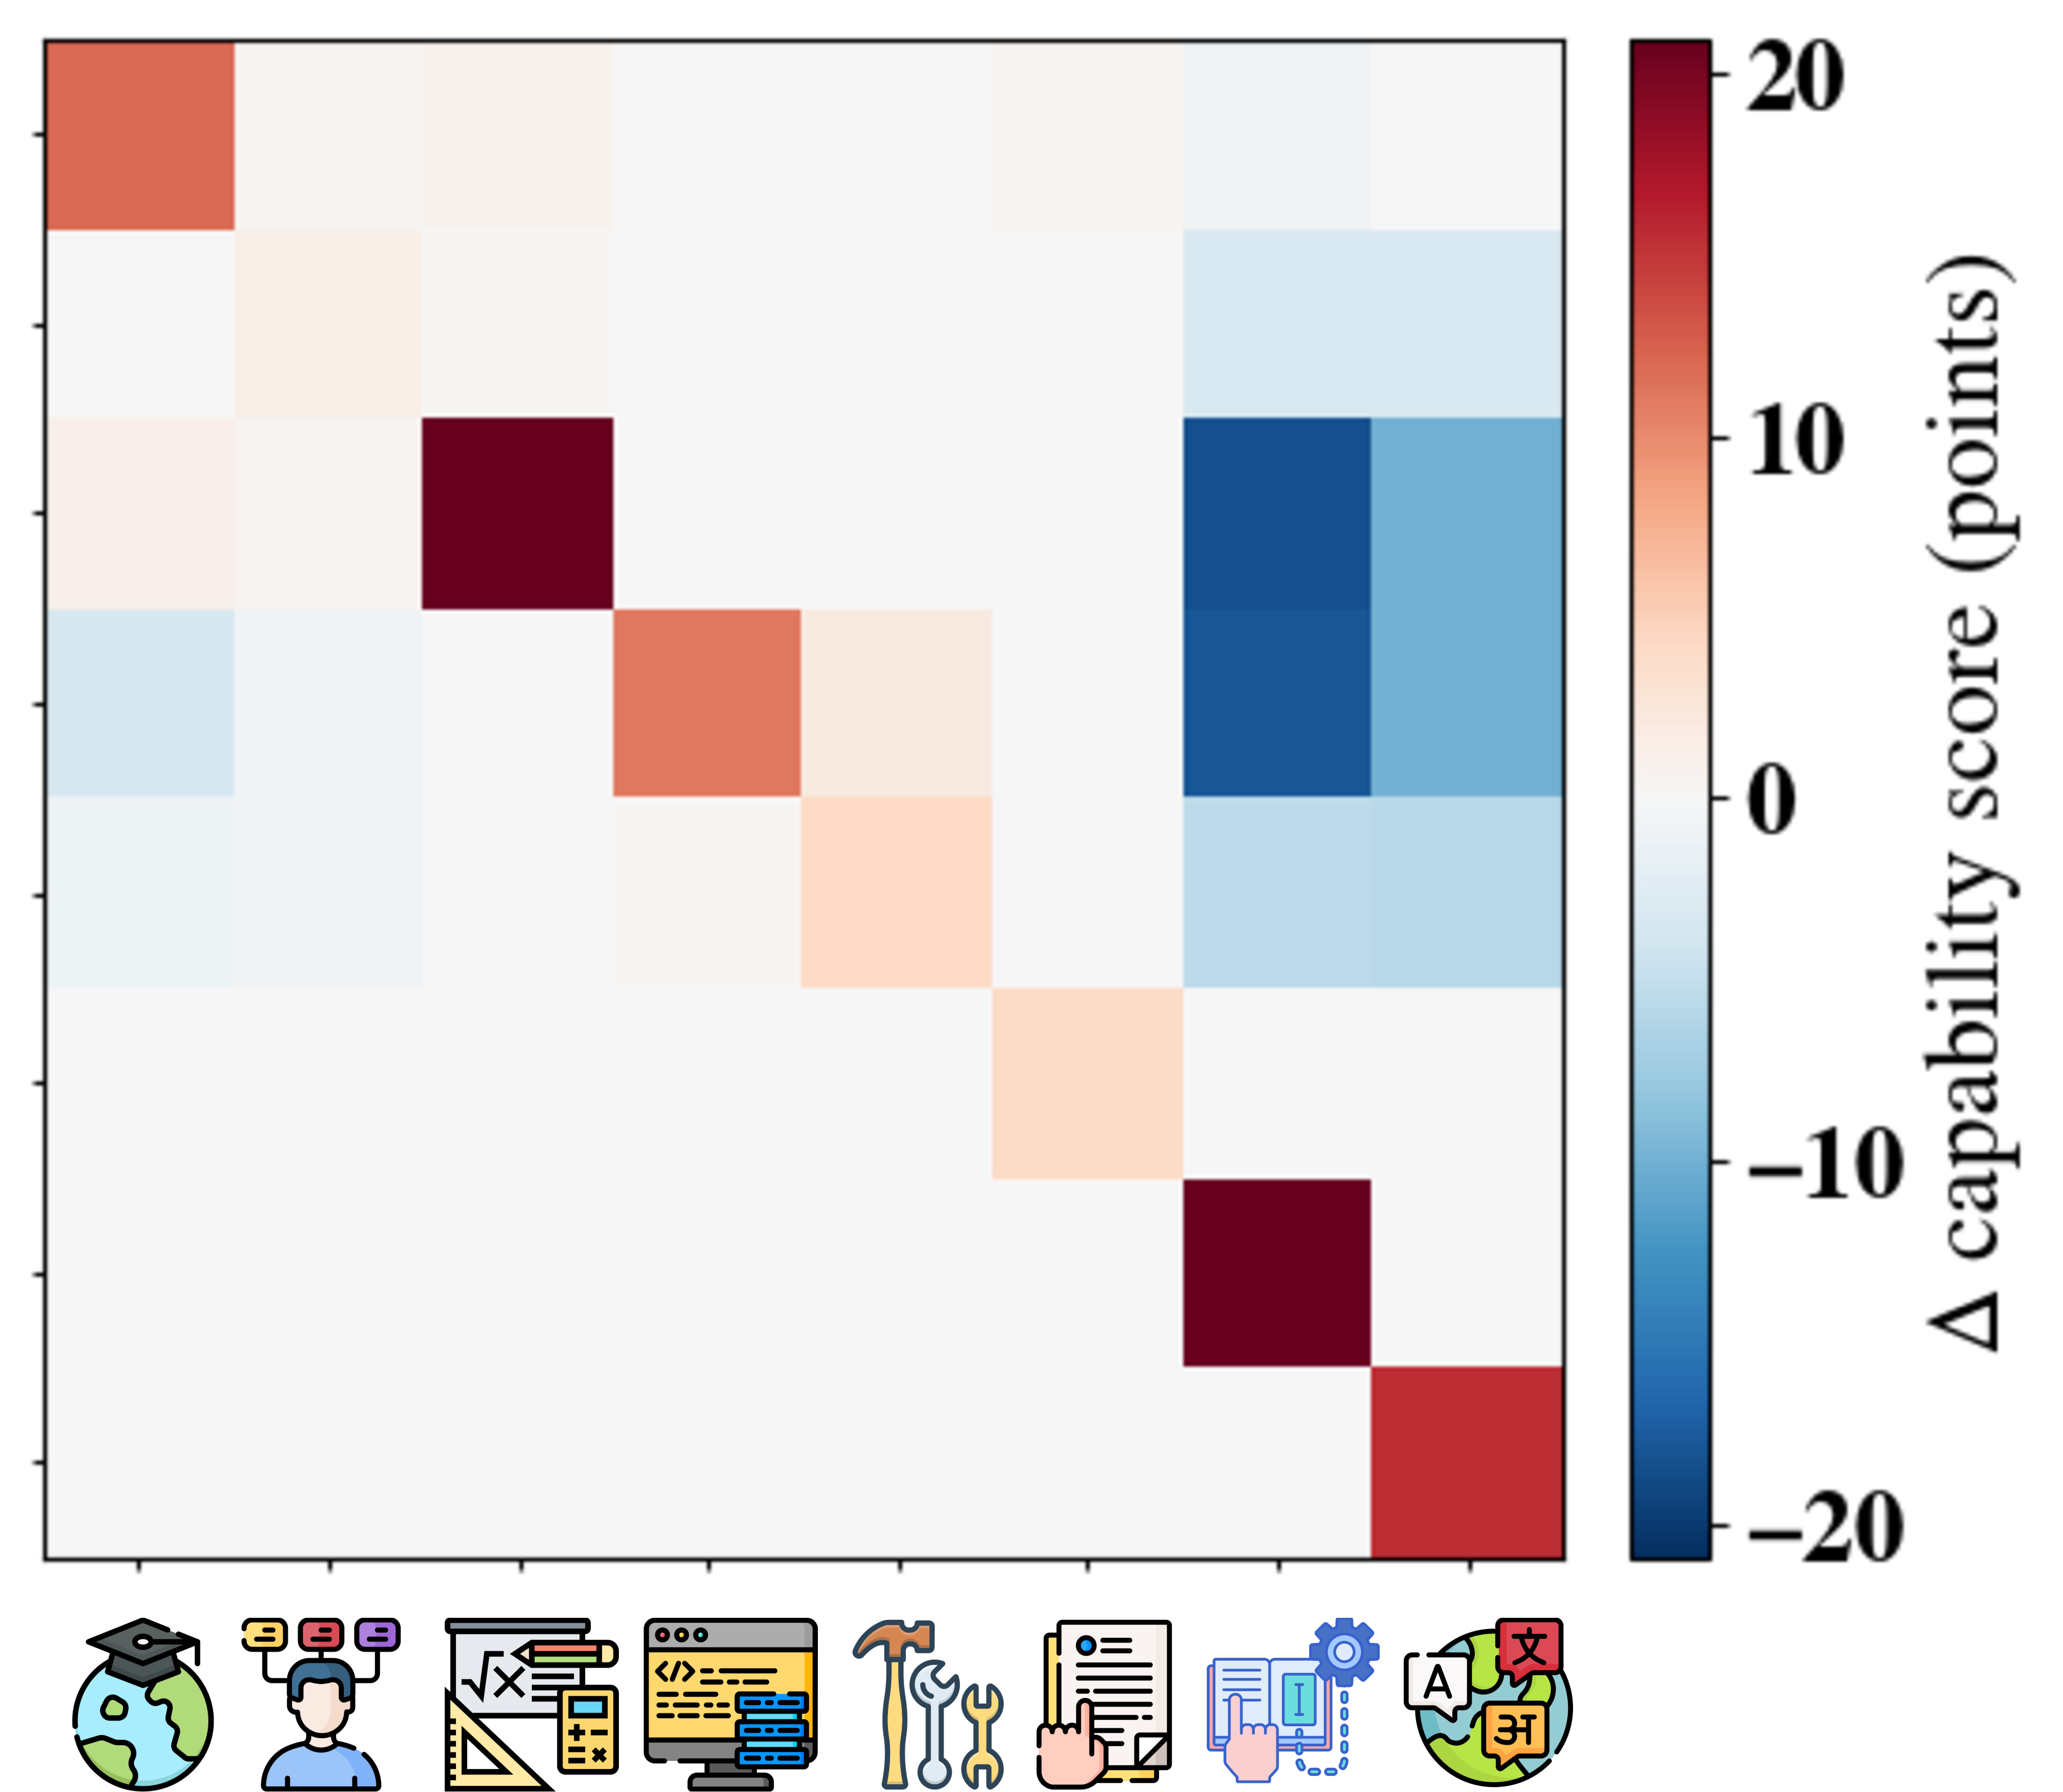
\includegraphics[height=72pt]{figure/heatmap_large.pdf}
    \caption{Large budget}
    \label{fig:heatmap_large}
  \end{subfigure}\hfill
  \begin{subfigure}[b]{0.306\linewidth}
    \centering
    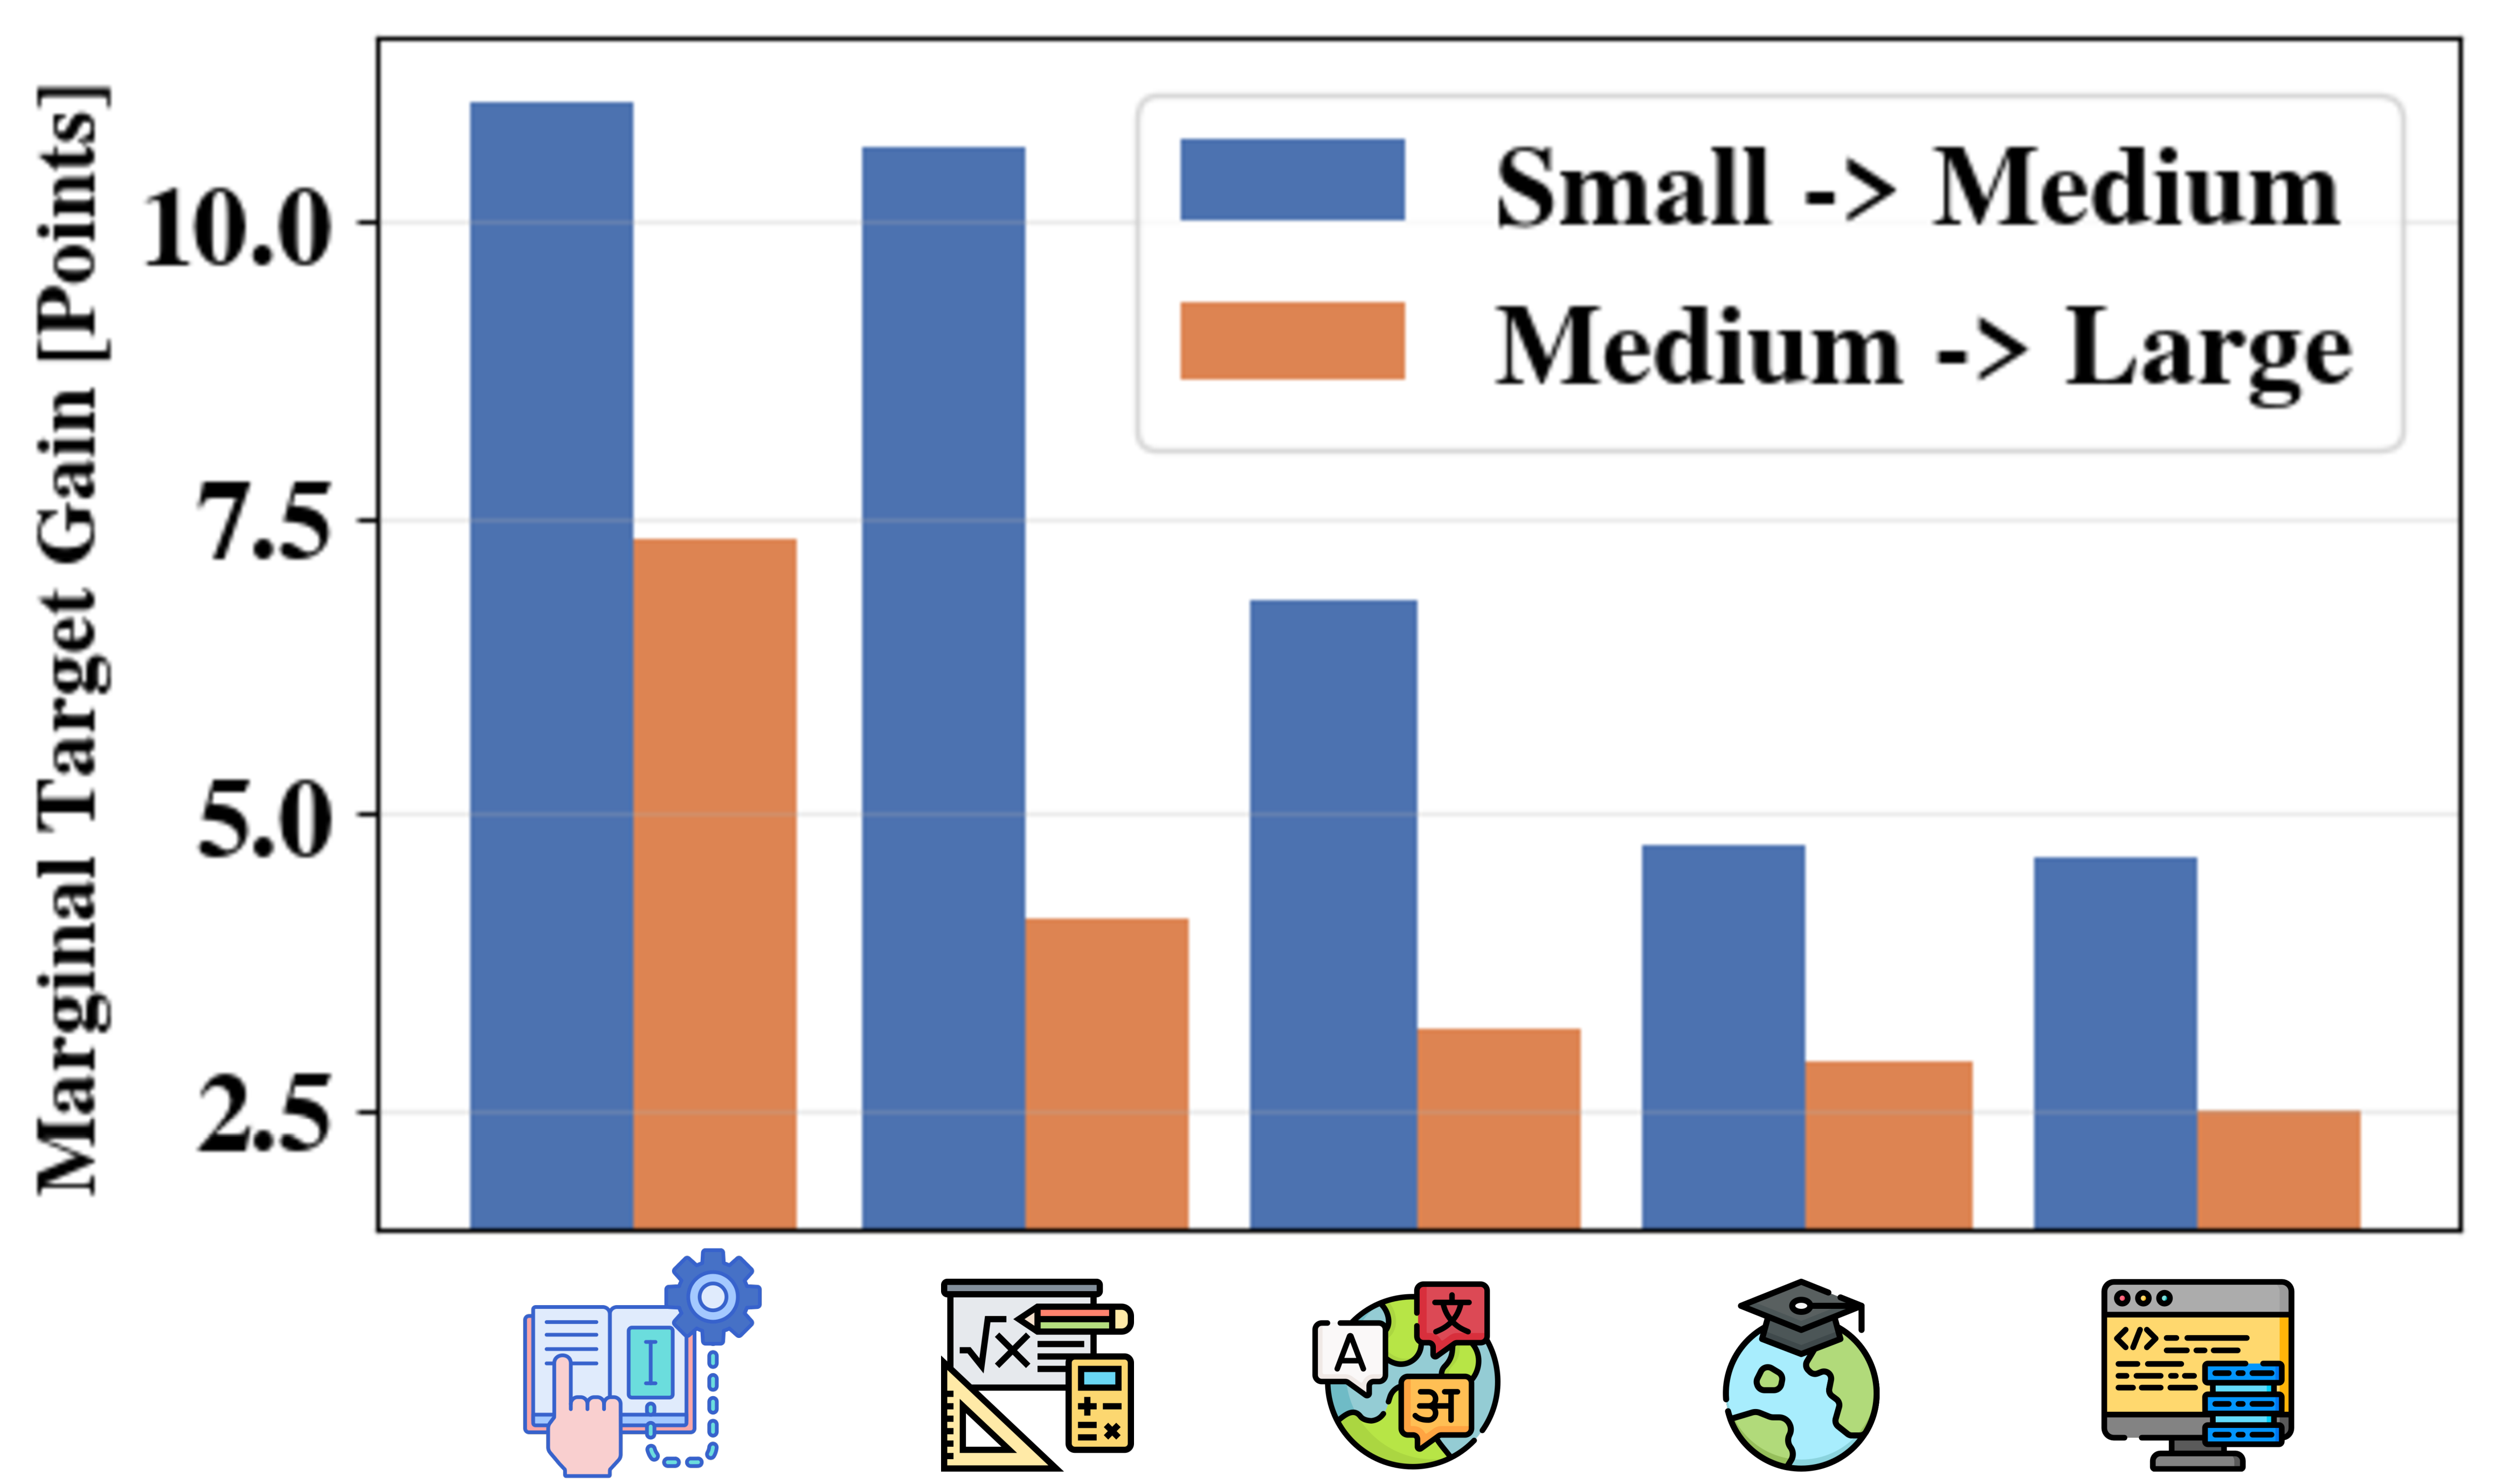
\includegraphics[height=72pt]{figure/Dimenshing.pdf}
    \caption{Diminishing returns}
    \label{fig:diminishing_returns}
  \end{subfigure}\hfill
  \begin{subfigure}[b]{0.270\linewidth}
    \centering
    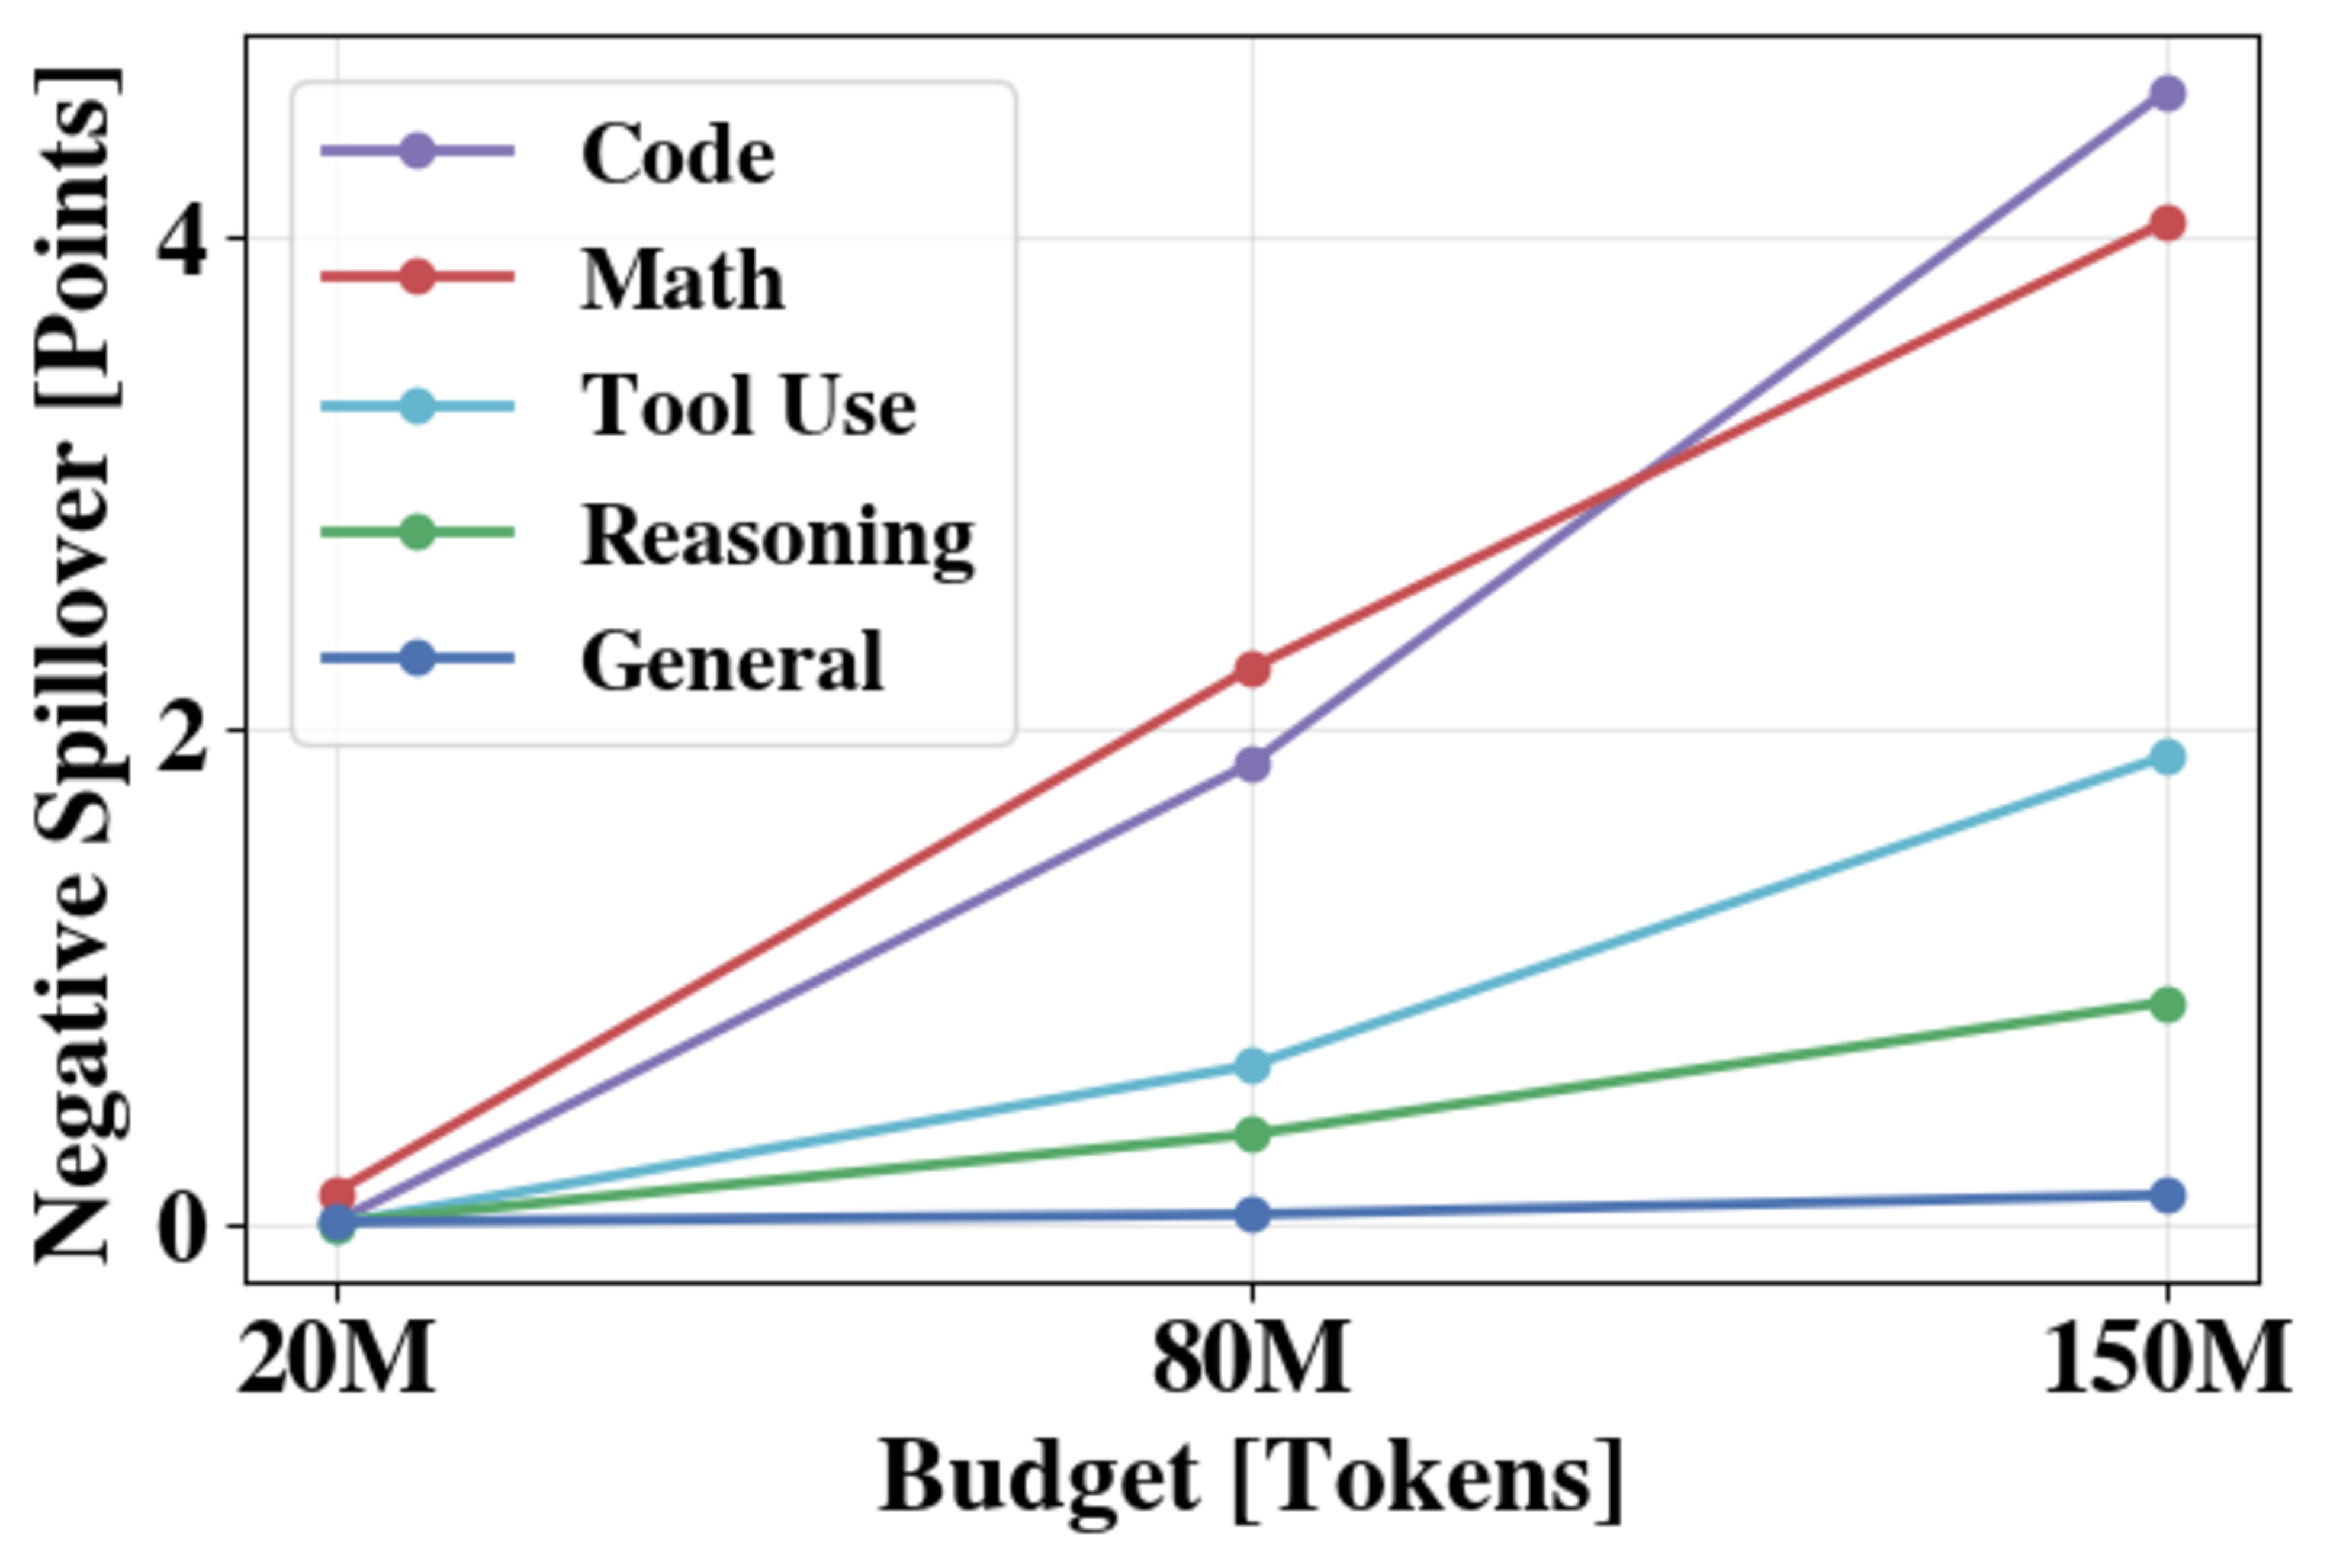
\includegraphics[height=72pt]{figure/spilover.pdf}
    \caption{Rising spillover}
    \label{fig:rising_spillover}
  \end{subfigure}
  \caption{\rev{Exploratory study. (a--b) Cross-capability transfer under
  single-capability distillation: larger budgets sharpen target gains but expose
  stronger negative transfer. (c--d) Budget waste: extra tokens yield smaller
  target gains while increasing harmful spillover to non-target capabilities.}}
  \label{fig:capability_transfer_heatmaps}
  \label{fig:budget_waste_mechanism}
  \vspace{-0.6em}
\end{figure}

\textbf{Observation 1: Distilling a specific capability redistributes performance across other capabilities in a budget-dependent manner.}
\rev{Figure~\ref{fig:capability_transfer_heatmaps}(a--b) shows the transfer
matrices at a small and a large budget. The off-diagonal mass is consistently
non-zero, so optimizing one capability moves the others rather than leaving
them unchanged, and the structure is budget-dependent: at small budgets the
changes are weak and diffuse, whereas at large budgets the diagonal sharpens and
negative off-diagonals appear for specific non-targets.}

\textbf{Observation 2: Capability distillation exhibits substantial budget waste
due to diminishing returns and negative spillover.}
\rev{For the strongest-improving targets, the marginal target gain of
20M$\rightarrow$80M is consistently larger than that of 80M$\rightarrow$150M
(\emph{diminishing returns}, Figure~\ref{fig:diminishing_returns}), while the
drop on non-target capabilities grows with the target's budget (\emph{negative
spillover}, Figure~\ref{fig:rising_spillover}). Beyond a capability-specific
knee point, extra tokens thus buy little target benefit and amplify
cross-capability degradation. Neither effect is new in isolation: off-target
drops are a form of catastrophic
forgetting~\citep{kirkpatrick2017overcoming,luo2023empirical}, and saturation
is ordinary diminishing returns. What allocation can exploit is their
\emph{structure}: transfer is signed, source-specific, and budget-dependent, so
a token's marginal value depends on where the budget has already gone.}

\rev{Effective distillation under a fixed budget must therefore reason jointly
about task-relevant capabilities, their interactions, and allocation. We
formalize this as a sequential budget allocation problem across interdependent capabilities, as follows:}

\begin{problem}[Budget allocation for interdependent capability distillation]\label{prob:budget_alloc}
Given a teacher model \( T \), an initial student model \( S_0 \), a downstream
task \( \tau \), and a total distillation budget \( B \), consider a sequential
distillation process over steps \( t=1,\ldots,T \) with cumulative cost not
exceeding \( B \). At each step \( t \), a capability allocation vector
\( \mathbf{w}_t\in\Delta_{|\mathcal{C}|} \) is selected and applied to update
the student, yielding \( S_t \). Let \( U_\tau(\cdot) \) \rev{be} the task-dependent utility function\rev{;} our target is to determine an allocation policy
\( \{\mathbf{w}_t\}_{t=1}^T \) that maximizes the performance of
the final student model:
\begin{equation}
\max_{\{\mathbf{w}_t\}_{t=1}^T}\ U_\tau\!\left(S_T\right), \
\text{s.t.}\;
\sum_{t=1}^T \mathrm{cost}\!\left(S_{t-1}\!\rightarrow\!S_t\right)\le B
\end{equation}
\end{problem}

\section{Methodology}
\label{sec:method}

ReAD treats Problem~\ref{prob:budget_alloc} as state-dependent budget allocation
over capabilities. At each step, it estimates task requirements, generates
capability-targeted teacher supervision, and uses an uncertainty-aware contextual
bandit to choose the next token allocation. As the student profile changes, ReAD
can shift budget away from saturated or high-spillover capabilities.
\rev{ReAD is \emph{off-policy} in the sense of \citet{agarwal2024gkd}: the
student trains on teacher completions to generated prompts and never samples
its own training sequences. The allocator is orthogonal to the inner objective,
and on-policy losses~\citep{gu2024minillm,ko2024distillm} could replace the
token-level loss in Section~\ref{sec:method:bandit} unchanged.}

\subsection{Identifying Task-Essential Capabilities}
\label{sec:method:essential}

\paragraph{Task requirement vector.}
For each downstream task $\tau$, ReAD constructs a task card
$\mathcal{D}^{\mathrm{spec}}_\tau$ from non-test data, containing a short task
description, input/output format, evaluation target, and a few representative
exemplars, with the test split reserved only for final reporting. From this
task card, ReAD estimates a requirement vector
$\mathbf{r}_\tau\in\Delta_{|\mathcal{C}|}$, where $r_{\tau,c}$ indicates how
useful capability $c$ is for improving the task utility $U_\tau(\cdot)$. We use
$\mathbf{r}_\tau$ as an actionable allocation prior: high-mass capabilities are
prioritized for improvement, and drops on these capabilities are treated as
harmful spillover. Since token allocations cannot be negative,
$\mathbf{r}_\tau$ is constrained to the simplex; negative sensitivities are
captured instead by signed capability changes and the spillover penalty in
Section~\ref{sec:method:bandit}.

\paragraph{Requirement identifier.}
We learn a lightweight identifier $g_\phi$ that maps the task card to the requirement vector $\mathbf{r}_\tau = g_\phi(\mathcal{D}^{\mathrm{spec}}_\tau) \in \Delta_{|\mathcal{C}|}$.
% \begin{equation}
% \mathbf{r}_\tau = g_\phi(\mathcal{D}^{\mathrm{spec}}_\tau) \in \Delta_{|\mathcal{C}|}.
% \label{eq:req_id}
% \end{equation}
The identifier is a small Transformer encoder over the task card, followed by a two-layer MLP and a softmax head. Since $\mathbf{r}_\tau$ is not directly observed, we supervise it through low-budget interventions in capability space.

\paragraph{Local supervision signal.}
Let $\mathbf{s}(S)\in\mathbb{R}^{|\mathcal{C}|}$ denote the measured capability profile of a student $S$, and write $U_\tau(S)=F_\tau(\mathbf{s}(S))$. For a small intervention that changes the profile from $\mathbf{s}$ to $\mathbf{s}+\Delta\mathbf{s}$,
\begin{equation}
F_\tau(\mathbf{s}+\Delta\mathbf{s})
=
F_\tau(\mathbf{s})+
\nabla_{\mathbf{s}}F_\tau(\mathbf{s})^\top\Delta\mathbf{s}
+o(\|\Delta\mathbf{s}\|),
\label{eq:taylor}
\end{equation}
so the utility change is locally approximated by
\begin{equation}
\Delta U_\tau
=
U_\tau(S')-U_\tau(S)
\approx
\nabla_{\mathbf{s}}F_\tau(\mathbf{s})^\top\Delta\mathbf{s}.
\label{eq:local_linear}
\end{equation}
Thus, $\mathbf{r}_\tau$ is trained as a simplex-constrained surrogate for the beneficial part of the local utility sensitivity, e.g., $\mathbf{r}_\tau\approx\Pi_\Delta([\nabla_{\mathbf{s}}F_\tau(\mathbf{s})]_+)$.

\paragraph{Offline pretraining.}
We construct an intervention set
$\mathcal{Z}=\{(\mathcal{D}^{\mathrm{spec}}_\tau,\Delta\mathbf{s}^{(m)}_\tau,\Delta U^{(m)}_\tau)\}_{\tau,m}$ from auxiliary tasks and non-test splits. For each task $\tau$, we sample sparse allocation vectors $\mathbf{w}^{(m)}\in\Delta_{|\mathcal{C}|}$ by choosing a support set $\mathcal{I}^{(m)}\subseteq\mathcal{C}$, sampling nonzero weights from a Dirichlet distribution, and renormalizing them. A short probe distillation under a small budget $b_{\mathrm{probe}}$ produces an intervened student $S^{(m)}$, from which we measure
\begin{equation}
\Delta U^{(m)}_\tau := U_\tau(S^{(m)})-U_\tau(S_0),
\qquad
\Delta\mathbf{s}^{(m)}_\tau := \mathbf{s}(S^{(m)})-\mathbf{s}(S_0).
\label{eq:probe_deltas}
\end{equation}
We pretrain $g_\phi$ by predicting the observed utility change from the induced capability change:
\begin{equation}
\min_\phi
\sum_{(\tau,m)}
\Big(\Delta U^{(m)}_\tau
- g_\phi(\mathcal{D}^{\mathrm{spec}}_\tau)^\top\Delta\mathbf{s}^{(m)}_\tau\Big)^2
+\lambda_{\mathrm{ent}}\,\mathcal{H}\!\left(g_\phi(\mathcal{D}^{\mathrm{spec}}_\tau)\right).
\label{eq:req_pretrain}
\end{equation}
The positive entropy penalty discourages near-uniform requirement vectors and makes the allocation prior more discriminative. At deployment time, ReAD computes $\mathbf{r}_\tau$ once and reuses it throughout the distillation run. Since the identifier is trained once and reused across tasks, it is not counted as part of the per-run student distillation budget.

\subsection{On-the-Fly Capability-Targeted Data Generation}
\label{sec:method-generator}

\paragraph{Capability-conditioned templates.}
Given $\mathbf{r}_\tau$, ReAD generates training examples on the fly from a capability-labeled template library. For each capability $c\in\mathcal{C}$, a template set $\mathcal{P}_c$ specifies an instruction scaffold, typed slots, and output-format constraints. Slot values are filled using deterministic seeds. The generator controls the form of teacher supervision

\paragraph{Difficulty scoring.}
For prompt $x$ in capability $c$, we compute a deterministic difficulty score
\begin{equation}
d_c(x)=\frac{1}{|\mathcal{F}_c|}\sum_{f\in\mathcal{F}_c}
\frac{f(x)-\min_{x'\in\mathcal{Q}_c} f(x')}
{\max_{x'\in\mathcal{Q}_c} f(x')-\min_{x'\in\mathcal{Q}_c} f(x')+\epsilon},
\label{eq:difficulty_score}
\end{equation}
where $\mathcal{F}_c$ is the set of capability-specific control factors and $\mathcal{Q}_c$ is a calibration prompt pool for capability $c$. For example, reasoning templates use factors such as the number of constraints, reasoning hops, and symbolic complexity; code templates use the number of required functions and tests; steerability templates use the number of rules and schema fields. We split each capability's calibration pool into easy, medium, and hard buckets by tertiles of $d_c(x)$.

\paragraph{Curriculum and sampling.}
At decision step $t$, ReAD samples a capability label according to the selected allocation $\mathbf{w}_t$, instantiates a prompt from the corresponding template set, queries the teacher $T$ for a completion $y$, and immediately distills on $(x,y)$. The curriculum only adjusts the within-capability difficulty mix: early steps emphasize easy and medium examples, while later steps increase the probability of hard examples. It does not choose the capability allocation. We also track recent template frequencies and cap each template's share so that no single scaffold dominates.

\subsection{Contextual Bandit for Capability Allocation}
\label{sec:method:bandit}

\paragraph{Decision loop.}
ReAD runs for $T_{\mathrm{step}}=20$ decision steps\rev{, with the bandit update, data resampling, and proxy refresh at every step (Section~\ref{subsec:exp_setup})}. At step $t$, the context summarizes the task requirement, current student profile, remaining budget, and recent allocation history:
\begin{equation}
\mathbf{x}_t=[\mathbf{r}_\tau;\mathbf{s}^{\mathrm{probe}}(S_t);b_t;\boldsymbol{\rho}_t],
\label{eq:bandit_context}
\end{equation}
where $\boldsymbol{\rho}_t$ stores a short record of recent allocations and observed gains. The profile $\mathbf{s}^{\mathrm{probe}}(S_t)$ is computed with a small fixed monitoring suite, while full held-out benchmark evaluation is used only for final reporting and coarse calibration.

\paragraph{Candidate allocations and distillation.}
At each step, ReAD selects an allocation $\mathbf{w}_t$ from a finite candidate set $\mathcal{A}(\tau)$ consisting of local perturbations around the previous allocation and sparse actions concentrated on the top-$k$ capabilities under $\mathbf{r}_\tau$. Weights are chosen from a fixed grid and renormalized to sum to one. Given $\mathbf{w}_t$, ReAD samples capability-targeted data and updates the student by minimizing $\mathcal{L}_{\mathrm{distill}}(\theta_t)
=-\mathbb{E}_{(x,y)}\sum_{j=1}^{|y|}
\log p_{\theta_t}(y_j\mid x,y_{<j})$ to produce $S_{t+1}$.
% \begin{equation}
% \mathcal{L}_{\mathrm{distill}}(\theta_t)
% =-\mathbb{E}_{(x,y)}\sum_{j=1}^{|y|}
% \log p_{\theta_t}(y_j\mid x,y_{<j}),
% \label{eq:distill_loss}
% \end{equation}

\paragraph{Proxy reward.}
After the update, ReAD measures the probe-profile change
$\Delta\mathbf{s}^{\mathrm{probe}}_t=\mathbf{s}^{\mathrm{probe}}(S_{t+1})-\mathbf{s}^{\mathrm{probe}}(S_t)$ and forms
\begin{equation}
\widehat{R}_t
=\mathbf{r}_\tau^\top\Delta\mathbf{s}^{\mathrm{probe}}_t
-\beta\,\mathrm{Spill}_t
-\lambda\,\mathrm{cost}_t, \quad\ \mathrm{Spill}_t=
\sum_{c\in\mathcal{C}_{\mathrm{ess}}}
 r_{\tau,c}\,[-\Delta s^{\mathrm{probe}}_{t,c}]_+
\label{eq:reward}
\end{equation}
Here $\mathcal{C}_{\mathrm{ess}}$ contains the top-$k$ capabilities under $\mathbf{r}_\tau$, and $\mathrm{cost}_t$ is the token budget consumed at the step. The first term rewards task-aligned capability gains, the second penalizes regressions on task-essential capabilities, and the third enforces budget awareness.

\paragraph{Reward model and UCB allocation.}
We append $(\mathbf{x}_t,\mathbf{w}_t,\widehat{R}_t)$ to a history buffer and train an ensemble of $J$ two-layer MLP reward regressors $\{h_{\eta_j}\}_{j=1}^J$. Each regressor maps $(\mathbf{x},\mathbf{w})$ to a scalar next-step reward and is trained on a bootstrap resample of the 10\% profiling split plus logged transitions from earlier steps, yielding about $3.2$k--$4.9$k examples per task in our experiments. For a candidate allocation $\mathbf{w}$, the ensemble mean and uncertainty are
\begin{equation}
\mu(\mathbf{x}_t,\mathbf{w})=\frac{1}{J}\sum_{j=1}^J h_{\eta_j}(\mathbf{x}_t,\mathbf{w}),
\quad
\sigma(\mathbf{x}_t,\mathbf{w})=
\sqrt{\frac{1}{J-1}\sum_{j=1}^J\big(h_{\eta_j}(\mathbf{x}_t,\mathbf{w})-\mu(\mathbf{x}_t,\mathbf{w})\big)^2}.
\label{eq:ensemble_mu_sigma}
\end{equation}
ReAD then selects the next allocation using an upper-confidence rule,
\begin{equation}
\mathbf{w}_{t+1}
=\arg\max_{\mathbf{w}\in\mathcal{A}(\tau)}
\mu(\mathbf{x}_{t+1},\mathbf{w})+\kappa\,\sigma(\mathbf{x}_{t+1},\mathbf{w}),
\label{eq:ucb}
\end{equation}
with $b_{t+1}=b_t-\mathrm{cost}_t$. At coarse development checkpoints, we fit an affine calibration from cumulative proxy reward to observed utility change and reduce exploration if the development utility stagnates. Unlike static mixture-regression approaches such as RegMix~\citep{liu2024regmix}, ReAD repeatedly re-estimates the best next allocation from the current student state and remaining budget.

\section{Theoretical Analysis}
\label{sec:theory}

This section provides a local theoretical account of ReAD's allocation problem.
We characterize cross-capability transfer under shared representations, show
when diminishing returns make continued allocation wasteful, and motivate
uncertainty-aware allocation under noisy reward estimates.

\subsection{Local Cross-Capability Transfer}
\label{subsec:theory_transfer_short}

Let $\theta_t\in\mathbb{R}^p$ denote the parameters of the student $S_t$, and let $\Delta\theta_t=\theta_t-\theta_{t-1}$. We analyze one decision step, which is the regime in which ReAD re-estimates its allocation.

\begin{assumption}[Mixture-structured update]
At interval $t$, given an allocation vector $\mathbf{w}_t\in\Delta_{|\mathcal{C}|}$, the expected update admits a local mixture approximation $\mathbb{E}[\Delta\theta_t\mid \mathbf{w}_t,\theta_{t-1}]
\approx
\sum_{c\in\mathcal{C}} w_{t,c}\,d_c(\theta_{t-1})$, where $d_c(\theta)$ is the capability-conditioned local update direction.
\end{assumption}

\begin{assumption}[Local capability readout]
The measured capability profile $\mathbf{s}(S)$ is represented locally as a differentiable function $\tilde{\mathbf{s}}(\theta)$. Near $\theta_{t-1}$,
\begin{equation}
\Delta s_{t,c}
=
[\mathbf{s}(S_t)]_c-[\mathbf{s}(S_{t-1})]_c
\approx
\nabla_\theta[\tilde{\mathbf{s}}(\theta_{t-1})]_c^\top\Delta\theta_t.
\label{eq:local_linear_short}
\end{equation}
\end{assumption}

\begin{proposition}[Local transfer decomposition]
Under the two local approximations above, the expected change in capability $c$ satisfies
\begin{equation}
\Delta s_{t,c}
\approx
\sum_{c'\in\mathcal{C}} w_{t,c'}\,\Gamma_{c,c'}(\theta_{t-1}),
\qquad
\Gamma_{c,c'}(\theta)
:=
\nabla_\theta[\tilde{\mathbf{s}}(\theta)]_c^\top d_{c'}(\theta).
\label{eq:transfer_decomp_short}
\end{equation}
\end{proposition}

\noindent\textit{Interpretation.}
\rev{$\Gamma$ is the local analogue of the empirical transfer matrix: diagonal
terms are intended gains, and off-diagonal terms are nonzero whenever the update
direction for $c'$ is not orthogonal to the readout direction of $c$, which is
expected under shared representations. This is why allocating budget to one
capability alters others at the decision-step level.}

\subsection{Budget Waste from Diminishing Returns}
\label{subsec:theory_diminish_short}

The previous subsection explains spillover. We now isolate diminishing returns with a simpler cumulative-budget proxy. Let $b_c\ge0$ be the total number of distillation tokens assigned to capability $c$, with $\sum_c b_c\le B$, and let $\mathbf{r}_\tau\in\Delta_{|\mathcal{C}|}$ be the task requirement vector.

\begin{assumption}[Concave task-aligned gains]
\label{assump:concave_gains_short}
For task $\tau$ and capability $c$, there is a nondecreasing concave gain function $G_{\tau,c}:\mathbb{R}_{\ge0}\to\mathbb{R}_{\ge0}$ such that $\mathbb{E}[U_\tau(S)-U_\tau(S_0)]
\approx
\sum_{c\in\mathcal{C}} r_{\tau,c}G_{\tau,c}(b_c)$ where $\sum_{c\in\mathcal{C}} b_c\le B$.
\end{assumption}

Consider a restricted distillation strategy that allocates budget only to a subset $\mathcal{K}\subseteq\mathcal{C}$:
\begin{equation}
\max_{\{b_c\ge0\}_{c\in\mathcal{K}}}
\sum_{c\in\mathcal{K}} r_{\tau,c}G_{\tau,c}(b_c)
\quad\mathrm{s.t.}\quad
\sum_{c\in\mathcal{K}} b_c\le B.
\label{eq:alloc_proxy_subset}
\end{equation}

\begin{proposition}[Weighted marginal gain criterion]
\label{prop:kkt_subset}
Any optimum $\{b_c^\star\}_{c\in\mathcal{K}}$ of Eq.~\eqref{eq:alloc_proxy_subset} equalizes weighted marginal gains among active capabilities: there exists $\nu^\star\ge0$ such that
\begin{equation}
r_{\tau,c}G'_{\tau,c}(b_c^\star)\le\nu^\star
\quad\forall c\in\mathcal{K},
\qquad
r_{\tau,c}G'_{\tau,c}(b_c^\star)=\nu^\star
\quad\text{if } b_c^\star>0.
\label{eq:kkt_subset}
\end{equation}
Moreover, in the single-capability case targeting $\bar c$, shifting an infinitesimal budget from $\bar c$ to another task-relevant capability $c'$ improves the proxy objective whenever $r_{\tau,c'}G'_{\tau,c'}(0)
>
r_{\tau,\bar c}G'_{\tau,\bar c}(b_{\bar c})$.
\end{proposition}

\noindent\textit{Implication for ReAD.}
\rev{This formalizes budget waste: once the target saturates, further tokens have
lower task-aligned marginal value than tokens assigned elsewhere. ReAD's reward
in Eq.~\eqref{eq:reward} is richer than this proxy because it also penalizes
observed spillover, so the allocator optimizes a step-level reward that
accounts for both diminishing returns and cross-capability degradation.}

\subsection{Why Uncertainty-Aware Allocation Helps}
\label{subsec:theory_ucb_short}

At step $t$, ReAD chooses from a finite action set $\mathcal{A}(\tau)$ using the ensemble mean $\mu(\mathbf{x}_t,\mathbf{w})$ and uncertainty $\sigma(\mathbf{x}_t,\mathbf{w})$ in Eq.~\eqref{eq:ucb}. Let $\overline{R}(\mathbf{x},\mathbf{w})
:=
\mathbb{E}[\widehat{R}_t\mid \mathbf{x}_t=\mathbf{x},\mathbf{w}_t=\mathbf{w}]$ be the conditional expected proxy reward\rev{ of action $\mathbf{w}$ in context $\mathbf{x}$}.

\begin{assumption}[Calibrated ensemble uncertainty]
\label{ass:calibrated_uncertainty}
For all encountered $(\mathbf{x}_t,\mathbf{w})$, with high probability, $|\mu(\mathbf{x}_t,\mathbf{w})-\overline{R}(\mathbf{x}_t,\mathbf{w})|
\le
\kappa\sigma(\mathbf{x}_t,\mathbf{w})$.
\end{assumption}

\begin{proposition}[Step-level regret bound]
Let $\mathbf{w}_t^\star\in\arg\max_{\mathbf{w}\in\mathcal{A}(\tau)}\overline{R}(\mathbf{x}_t,\mathbf{w})$. Under Assumption~\ref{ass:calibrated_uncertainty}, the action selected by Eq.~\eqref{eq:ucb} satisfies $\overline{R}(\mathbf{x}_t,\mathbf{w}_t^\star)
-
\overline{R}(\mathbf{x}_t,\mathbf{w}_t)
\le
2\kappa\sigma(\mathbf{x}_t,\mathbf{w}_t)$.
\end{proposition}

\noindent\textit{Proof sketch.}
By calibration, the true reward of any action is at most its upper confidence score, and the selected action maximizes this score. Applying the same calibration inequality to the selected action yields the bound. This result does not imply a global optimum for nonconvex fine-tuning; it justifies the local ranking rule used by ReAD at each budget step.

\section{Experimental Setting}
\label{subsec:exp_setup}

\textbf{Models and budgets.}
We mainly distill Llama-3.3-70B-Instruct into Llama-3.1-8B-Instruct, and report
Qwen2.5-72B-Instruct to Qwen2.5-14B-Instruct results in
Appendix~\ref{sec:app_experiment}. All methods use the same student checkpoint,
training recipe, and $20$M/$150$M distillation-token budgets.

\textbf{Evaluation protocol.}
We evaluate eight capabilities using Appendix
Table~\ref{tab:capabilities-benchmarks}. For each benchmark, 10\% of non-test
data is used for profiling, requirement inference, and allocation updates; the
held-out split is reserved for final reporting. Generation uses temperature $0$
with the same prompt template across methods. We report mean $\pm$ standard
deviation over three seeds.

\textbf{Baselines.}
For each capability, we build a held-out-filtered distillation pool from its
benchmark prompts. For multi-dataset capabilities, we use balanced dataset-level
sampling. The six main baselines combine three teacher signals---final response
(Resp), chain-of-thought plus response (CoT), and token-level logits (Logit)---
with two objectives, SFT and KD. Each baseline is one-hot at the capability
level, spending the full budget on the target-capability pool.
\rev{We also compare against four allocation baselines that share ReAD's
generator, teacher, and budget and differ only in how $\mathbf{w}_t$ is chosen
(Table~\ref{tab:budget_diagnostics}): \emph{Uniform static}
($\mathbf{w}_t=\mathbf{1}/|\mathcal{C}|$), \emph{Task-static mix}
($\mathbf{w}_t=\mathbf{r}_\tau$), \emph{Greedy one-step} (re-selects
$\mathbf{w}_t$ each step by the ensemble mean alone, $\kappa=0$), and
\emph{Grid-searched} (best fixed allocation in $\mathcal{A}(\tau)$ on the
profiling split). These are the matched reference points for adaptive allocation.}

\textbf{ReAD implementation.}
ReAD runs for $20$ decision steps, with bandit updates, proxy refreshes, and data
resampling every $1.0$M tokens in the $20$M setting and every $7.5$M tokens in
the $150$M setting. Proxy refresh adds 3.12\% wall-clock overhead, the full online loop adds
5.63\%, and the reusable requirement identifier costs 3.79 GPU-hours to train
once.
\rev{\textbf{Cost accounting.} $B$ counts the teacher-generated tokens the
student is trained on and is identical for all methods. Two ReAD-specific costs
fall outside $B$ and are reported separately rather than folded into it: the
identifier is trained once from auxiliary tasks and reused for every task and
budget, so its 3.79 GPU-hours are amortized, and the fixed probe suite is the
3.12\% overhead above.}


\section{Experiments}
\label{sec:exp}

We study four questions: \textbf{RQ1} utility gains under the same budget;
\textbf{RQ2} reduced waste and spillover; \textbf{RQ3} the value of adaptive
bandit scheduling over static or greedy alternatives; and \textbf{RQ4}
transfer beyond capability-aligned benchmarks.

\begin{table*}[t]
\centering
\tiny
\setlength\tabcolsep{1pt}
\caption{Capability profile under a 20M-token budget on Llama. ReAD achieves the strongest average profile while using the same student initialization and token budget as all baselines.}
\begin{tabular}{lcccccccc}
\toprule
\textbf{Method} &
\textbf{General} &
\textbf{Steer.} &
\textbf{Reason.} &
\textbf{Math} &
\textbf{Code} &
\textbf{Tool} &
\textbf{LCU} &
\textbf{Multi.} \\
\midrule
Teacher only &
$48.13\pm0.35$ & $89.98\pm0.40$ & $10.51\pm0.12$ & $48.34\pm0.55$ &
$88.40\pm0.70$ & $31.90\pm0.45$ & $36.20\pm0.40$ & $91.10\pm0.55$ \\
Student only &
$31.09\pm0.40$ & $49.22\pm0.55$ & $8.72\pm0.15$ & $15.56\pm0.60$ &
$72.60\pm0.95$ & $25.83\pm0.60$ & $30.40\pm0.45$ & $68.90\pm0.80$ \\
\midrule
Resp-SFT & $33.28\pm0.47$ & $52.84\pm0.71$ & $9.05\pm0.18$ & $17.12\pm0.83$ & $74.06\pm1.09$ & $26.92\pm0.78$ & $31.28\pm0.51$ & $70.02\pm0.93$ \\
CoT-SFT & $33.02\pm0.52$ & $52.16\pm0.76$ & $9.46\pm0.14$ & $18.58\pm0.77$ & $73.82\pm1.02$ & $26.81\pm0.74$ & $31.19\pm0.57$ & $69.78\pm0.88$ \\
Logit-SFT & $33.61\pm0.44$ & $53.04\pm0.69$ & $9.12\pm0.17$ & $17.63\pm0.79$ & $74.48\pm1.15$ & $27.03\pm0.70$ & $31.42\pm0.53$ & $70.21\pm0.90$ \\
Resp-KD & $33.83\pm0.50$ & $53.62\pm0.73$ & $9.18\pm0.16$ & $17.84\pm0.74$ & $74.23\pm1.07$ & $27.18\pm0.76$ & $31.58\pm0.55$ & $70.48\pm0.95$ \\
CoT-KD & $33.46\pm0.46$ & $52.98\pm0.78$ & $9.62\pm0.13$ & $19.34\pm0.72$ & $74.03\pm1.10$ & $27.06\pm0.72$ & $31.47\pm0.58$ & $70.08\pm0.89$ \\
Logit-KD & $34.02\pm0.43$ & $54.21\pm0.66$ & $9.25\pm0.15$ & $18.20\pm0.76$ & $74.62\pm1.12$ & $27.41\pm0.69$ & $31.72\pm0.50$ & $70.81\pm0.91$ \\
\midrule
\textbf{ReAD} &
$\mathbf{35.02\pm0.41}$ & $\mathbf{58.03\pm0.61}$ & $\mathbf{10.01\pm0.12}$ & $\mathbf{21.06\pm0.68}$ &
$\mathbf{77.06\pm0.97}$ & $\mathbf{29.82\pm0.64}$ & $\mathbf{33.58\pm0.49}$ & $\mathbf{73.04\pm0.84}$ \\
\bottomrule
\end{tabular}
\label{tab:llama_20m}
\end{table*}

\begin{figure}[t]
  \centering
  
\includegraphics[width=\columnwidth]{figure/rq2_legend.pdf}
  \vspace{-1.5em}

  \begin{subfigure}[t]{0.24\columnwidth}
    \centering
    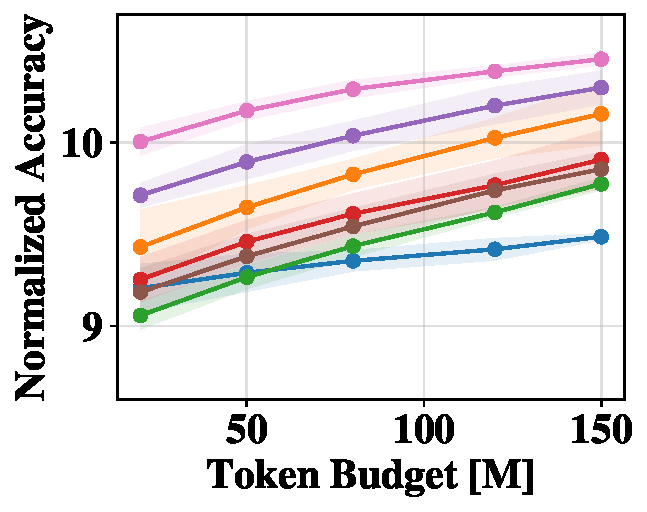
\includegraphics[width=\linewidth]{figure/rq2_lineplot_reasoning.pdf}
    \caption{Reasoning}
    \label{fig:r2_reason}
  \end{subfigure}
  \hfill
  \begin{subfigure}[t]{0.24\columnwidth}
    \centering
    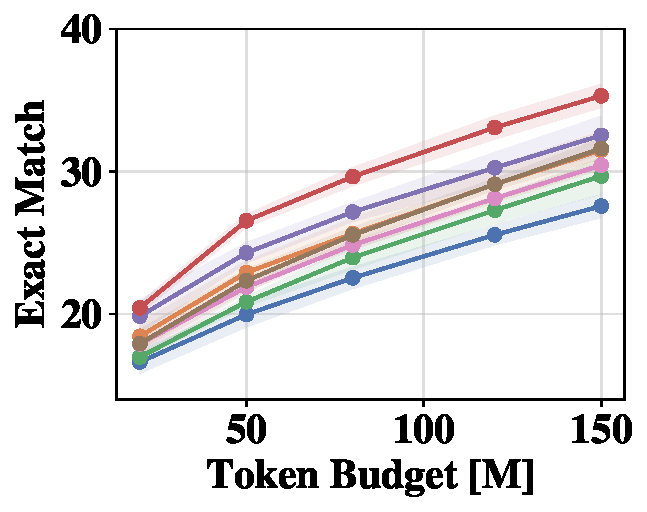
\includegraphics[width=\linewidth]{figure/rq2_lineplot_math.pdf}
    \caption{Math}
    \label{fig:r2_math}
  \end{subfigure}
  \hfill
  \begin{subfigure}[t]{0.24\columnwidth}
    \centering
    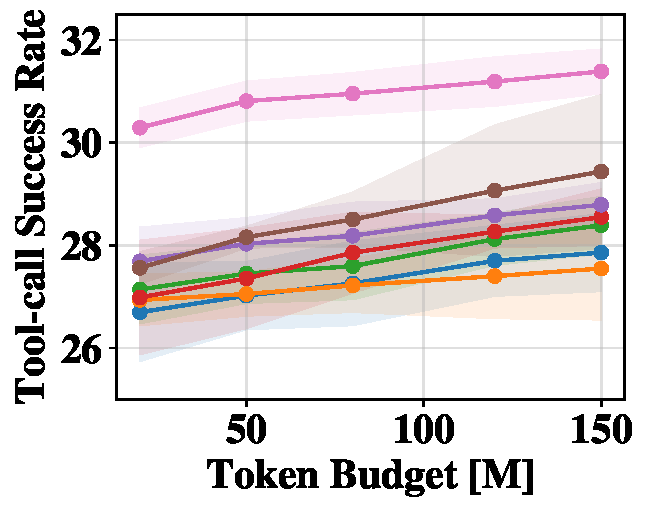
\includegraphics[width=\linewidth]{figure/rq2_lineplot_tool_use.pdf}
    \caption{Tool Use}
    \label{fig:r2_tool}
  \end{subfigure}
  \hfill
  \begin{subfigure}[t]{0.24\columnwidth}
    \centering
    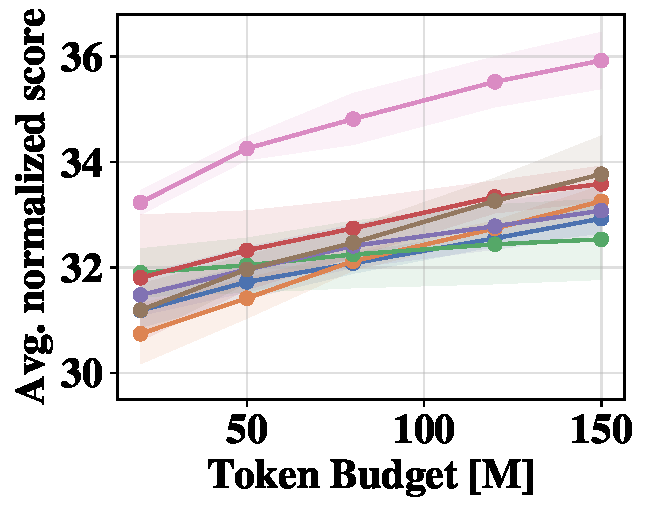
\includegraphics[width=\linewidth]{figure/rq2_lineplot_lcu.pdf}
    \caption{LCU}
    \label{fig:r2_lcu}
  \end{subfigure}

  \caption{Performance versus token budget for four bottleneck capabilities. Curves show mean $\pm$ standard deviation over three seeds.}
  \label{fig:rq2_budget}
  \vspace{-0.8em}
\end{figure}

\subsection{Results and Analysis}
\label{subsec:exp_results}

\paragraph{RQ1: Utility under a fixed budget.}
Table~\ref{tab:llama_20m} shows that ReAD achieves the strongest capability
profile at $20$M tokens\rev{, outperforming the six one-hot baselines on every
capability}. The gains
are especially pronounced on bottleneck capabilities such as Steerability, Math,
Tool Use, and LCU. \rev{Since each one-hot baseline spends the whole budget on one capability,
this isolates the value of distributing the budget at all; the matched
comparison for \emph{how} to distribute it is Table~\ref{tab:budget_diagnostics}(b) (RQ3).} The $150$M Llama results and Qwen results in
Appendix~\ref{sec:app_experiment} show the same ordering, suggesting that the
improvement is not tied to a single teacher--student pair.

\paragraph{RQ2: Budget efficiency.}
Figure~\ref{fig:rq2_budget} reports budget-scaling curves for Reasoning, Math,
Tool Use, and LCU. ReAD achieves higher performance at the same budget and
maintains the strongest scaling trend, indicating that adaptive allocation
reduces wasted tokens on low-marginal-return updates.

\begin{table}[t]
  \centering
  \captionsetup{font=small, width=0.96\linewidth, skip=3pt}
  \caption{\rev{\textbf{Budget-allocation diagnostics.} (a) 150M-token
gain--spillover trade-off from the capability transfer matrix: ReAD keeps
near-best on-target gain with much less off-target degradation. (b)
Matched-budget allocation schedules under the same generator.}}
  \label{tab:budget_diagnostics}
  \vspace{-0.4em}

  \footnotesize
  \setlength{\tabcolsep}{2.2pt}
  \renewcommand{\arraystretch}{0.94}

  \begin{subtable}[t]{0.55\linewidth}
    \centering
    \caption*{\textbf{(a) Harmful transfer at 150M}}
    \begin{tabular}{@{}lccc@{}}
      \toprule
      \textbf{Method} & \textbf{On-tgt $\uparrow$} & \textbf{Off-tgt $\Delta\uparrow$} & \textbf{Neg. $\downarrow$} \\
      \midrule
      Single-cap. KD
        & $\mathbf{4.79{\pm}0.29}$
        & $-1.57{\pm}0.21$
        & $0.43{\pm}0.03$ \\
      Task-static mix
        & $4.61{\pm}0.25$
        & $-0.87{\pm}0.17$
        & $0.29{\pm}0.03$ \\
      Greedy one-step
        & $4.72{\pm}0.23$ % placeholder: replace with measured value
        & $-0.94{\pm}0.19$ % placeholder: replace with measured value
        & $0.31{\pm}0.03$ % placeholder: replace with measured value
        \\
      Grid-searched
        & $4.66{\pm}0.24$ % placeholder: replace with measured value
        & $-0.71{\pm}0.16$ % placeholder: replace with measured value
        & $0.25{\pm}0.03$ % placeholder: replace with measured value
        \\
      \textbf{ReAD}
        & $4.79{\pm}0.24$
        & $\mathbf{-0.38{\pm}0.12}$
        & $\mathbf{0.17{\pm}0.02}$ \\
      \bottomrule
    \end{tabular}
  \end{subtable}
  \hfill
  \begin{subtable}[t]{0.42\linewidth}
    \centering
    \caption*{\textbf{(b) Allocation schedules}}
    \begin{tabular}{@{}lcc@{}}
      \toprule
      \textbf{Method} & \textbf{20M $\uparrow$} & \textbf{150M $\uparrow$} \\
      \midrule
      Uniform static
        & $60.94{\pm}0.48$
        & $64.73{\pm}0.36$ \\
      Task-static mix
        & $61.71{\pm}0.43$
        & $65.52{\pm}0.33$ \\
      Greedy one-step
        & $62.03{\pm}0.41$
        & $66.01{\pm}0.30$ \\
      Grid-searched
        & $61.88{\pm}0.42$
        & $65.81{\pm}0.31$ \\
      \textbf{ReAD}
        & $\mathbf{63.04{\pm}0.39}$
        & $\mathbf{67.21{\pm}0.28}$ \\
      \bottomrule
    \end{tabular}
  \end{subtable}

  \vspace{-1.6em}
\end{table}

\paragraph{RQ2: Gain--spillover trade-off.}
Table~\ref{tab:budget_diagnostics}(a) shows that ReAD improves the
gain--spillover trade-off. Single-capability KD achieves strong target gains but
causes larger off-target degradation, while static mixing reduces spillover at
the cost of weaker target improvement. ReAD better balances the two: it keeps
strong on-target gains while suppressing negative transfer across
non-target capabilities.

\paragraph{RQ3: Adaptive scheduling.}
Table~\ref{tab:budget_diagnostics}(b) compares ReAD with stronger allocation
baselines under the same generator and token budgets. Static schedules cannot
adapt once marginal returns and spillover change during training, while the
greedy heuristic ignores uncertainty and remaining budget. ReAD outperforms
both, with a larger margin at $150$M where saturation and spillover are stronger.
\rev{These margins are smaller than those over one-hot baselines ($+1.0$/$+1.2$
over Greedy one-step and $+1.2$/$+1.4$ over Grid-searched at $20$M/$150$M, with
seed standard deviations of $0.3$--$0.4$), as every allocation baseline already
mixes capabilities; the remaining gain is the value of re-estimating the mix as
the student and the remaining budget change.}

\begin{wrapfigure}[8]{r}{0.42\textwidth}
  \vspace{-1.6em}
  \centering
  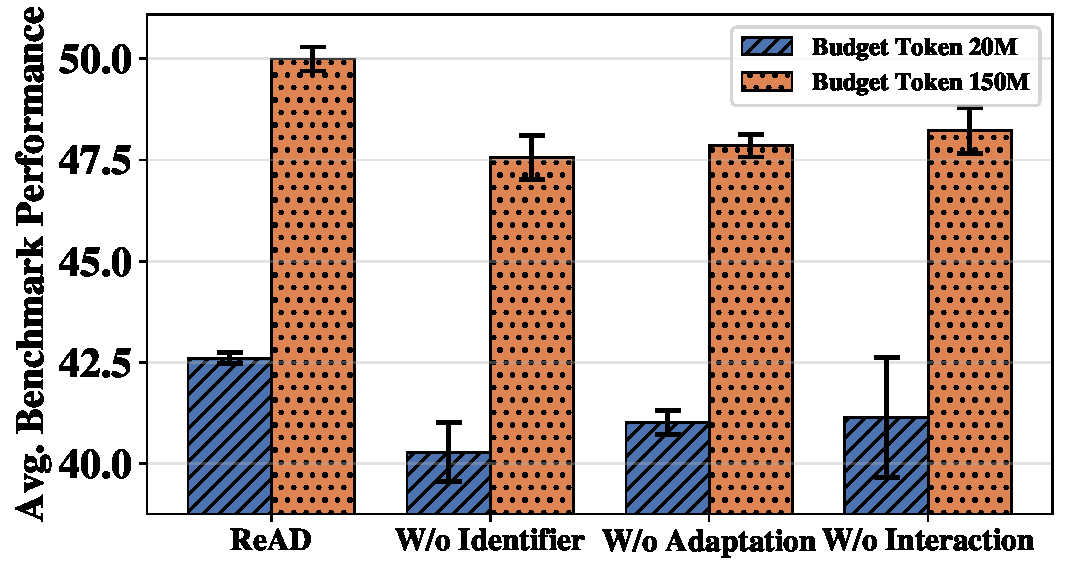
\includegraphics[width=0.40\textwidth]{figure/rq3_ablation_avgmetric_20m_150m.pdf}
  \caption{Ablation of ReAD components.}
  \label{fig:rq3_ablation}
  \vspace{-1.4em}
\end{wrapfigure}

\paragraph{Component ablation.}
We ablate ReAD by removing one component while fixing the teacher, student,
prompt pools, training recipe, and budget. Removing requirement identification
makes the allocation uniform; removing adaptation uses a fixed allocation; and
removing interaction awareness drops the spillover penalty.
Figure~\ref{fig:rq3_ablation} shows that identification and adaptation drive the
largest gains, while interaction modeling provides additional improvement by
reducing harmful transfer.

\paragraph{RQ4: Transfer beyond aligned benchmarks.}
Finally, we evaluate ReAD on held-out XSTest~\citep{rottger2024xstest} using the same requirement
identifier and allocation pipeline without adding a new capability head. ReAD
improves both safe-refusal and unsafe-refusal metrics over the best SFT/KD
baseline; full results are reported in Appendix Table~\ref{tab:xstest}.
\section{Conclusions}
\label{sec:con}

\rev{We study how to allocate a fixed distillation budget across capability-targeted supervision to improve a specified target capability. ReAD combines a task-conditioned allocation prior, on-the-fly teacher supervision, and an uncertainty-aware contextual bandit. Under the same budget, it achieves higher on-target scores than target-only baselines, improves over static and greedy schedules with a matched generator, and shows smaller off-target declines than single-capability distillation. Its proxy reward may deviate from true task utility, and its efficiency figures are interpolation-based estimates from two budgets; validating both is left to future work. More broadly, our results indicate that how supervision is allocated across capabilities, and not only how much of it is used, shapes both what a distilled student learns and what it loses along the way.}
% demonstrating the value of treating capability distillation as a budgeted control problem that explicitly models capability interdependence.

% ============================================================
% Required / recommended statements (ICLR 2027 Author Guidelines):
% placed at the end of the main text, before the references;
% none of them counts toward the page limit.
% ============================================================
% ICLR 2027: AI use statement (required), Ethics statement and
% Reproducibility statement (recommended). All three go at the end of the
% main text, before the references, and do not count toward the page limit.

\keepwithnext{5\baselineskip}
\subsection*{AI use statement}

\rev{We used generative AI tools to help implement parts of the experimental code
and to edit the grammar and wording of the manuscript, but not to design the
method or experiments, derive the theory, generate data, or interpret results.
The authors verified all AI-assisted content and take full responsibility for the final paper.}

\subsection*{Reproducibility statement}

\rev{Sections~\ref{sec:method} and~\ref{subsec:exp_setup} describe the method and
setup, Appendices~\ref{sec:bench_datasets}--\ref{sec:app_experiment} give the
benchmarks, proofs, and further results, and all numbers are means and standard
deviations over three seeds. Code and configurations are available at
\url{https://anonymous.4open.science/r/ReAD-62B7}.}


% ============================================================
% References
% ============================================================
\bibliographystyle{iclr2027_conference}
\bibliography{ref}

\appendix
% appendix only: allow up to three top floats per page so tables do not pile up at the end
\setcounter{topnumber}{3}\setcounter{totalnumber}{5}\renewcommand{\topfraction}{0.9}\renewcommand{\textfraction}{0.08}

\newpage
\section*{Technical Appendices and Supplementary Material}


\section{Benchmark Datasets}\label{sec:bench_datasets}

Table~\ref{tab:capabilities-benchmarks} summarizes the benchmark suite used to
evaluate each capability. For capabilities associated with multiple benchmarks,
we report the average score across the listed benchmarks.


\begin{table}[h]
  \centering
  \caption{Benchmark suite for evaluating LLM capabilities.}
  \label{tab:capabilities-benchmarks}
  \small
  \setlength{\tabcolsep}{4pt}
  \renewcommand{\arraystretch}{0.95}

  \begin{tabularx}{\linewidth}{@{}
    >{\raggedright\arraybackslash}p{0.20\linewidth}
    >{\raggedright\arraybackslash}p{0.36\linewidth}
    >{\raggedright\arraybackslash}X
  @{}}
    \toprule
    \textbf{Capability} & \textbf{Benchmarks} & \textbf{Metric} \\
    \midrule
    General      & MMLU-Pro, BIG       & Accuracy \\
    Steerability & IFEval, FollowEval  & Instruction-following accuracy \\
    Reasoning    & GPQA, ARC-Challenge & Normalized accuracy \\
    Math         & MATH Hard, GSM8K    & Exact match \\
    Code         & HumanEval, MBPP     & Pass@1 \\
    Tool Use     & BFCL V4, ToolBench  & Tool-call success rate \\
    LCU          & LongBench           & Average normalized score \\
    Multilingual & XCOPA, MGSM         & Macro accuracy \\
    \bottomrule
  \end{tabularx}
\end{table}

\begin{itemize}
    \item \textbf{MMLU-Pro}~\citep{wang2024mmluprorobustchallengingmultitask} tests broad knowledge and problem-solving across many academic subjects using multiple-choice questions. 
    \item \textbf{BIG-bench (BIG)}~\citep{suzgun2022challenging} is a large collection of diverse tasks designed to probe general reasoning and knowledge beyond standard exams.
    \item \textbf{IFEval}~\citep{zhou2023instructionfollowing} measures instruction following by checking whether model outputs satisfy explicit, verifiable constraints in the prompt.
    \item \textbf{FollowEval}~\citep{jing2023followeval} evaluates how well a model follows user instructions under varied formats and constraint types, complementing IFEval with broader instruction patterns.
    \item \textbf{GPQA}~\citep{rein2024gpqa} is a graduate-level question answering benchmark that stresses hard scientific reasoning with high-quality, expert-written questions.
    \item \textbf{ARC-Challenge}~\citep{Clark2018ThinkYH} contains difficult grade-school science questions that require multi-step reasoning and commonsense beyond keyword matching.
    \item \textbf{MATH Hard}~\citep{hendrycksmath2021} is a challenging subset of competition-style math problems and is scored by exact final-answer match.
    \item \textbf{GSM8K}~\citep{cobbe2021training} focuses on grade-school math word problems that require intermediate reasoning steps, also scored by exact final-answer match.
    \item \textbf{HumanEval}~\citep{chen2021codex} evaluates code generation via functional correctness on hand-written programming problems, reported as Pass@1.
    \item \textbf{MBPP}~\citep{austin2021program} is a Python programming benchmark with short programming tasks and unit tests, also evaluated by Pass@1.
    \item \textbf{BFCL V4}~\citep{berkeley-function-calling-leaderboard} measures tool-use ability by checking whether the model can produce correct function calls under realistic tool specifications.
    \item \textbf{ToolBench}~\citep{xu2023tool} evaluates tool use in more complex, multi-tool scenarios and is scored by tool-call success rate.
    \item \textbf{LongBench}~\citep{bai2024longbench} evaluates long-context understanding across multiple long-input tasks and reports an average normalized score.
    \item \textbf{XCOPA}~\citep{ponti2020xcopa} tests multilingual causal commonsense reasoning across languages and is reported using macro accuracy.
    \item \textbf{MGSM}~\citep{shi2022language} is a multilingual version of grade-school math and is evaluated by macro accuracy across languages.
\end{itemize}

\section{Empirical Study Setting}\label{sec:app_em}

We study capability interactions under a fixed distillation budget by distilling a student model toward one target capability at a time and then evaluating the resulting student on \emph{all} capabilities in Table~\ref{tab:capabilities-benchmarks}. 
For each capability, we build a capability-specific distillation pool from the corresponding benchmark prompts, excluding any held-out evaluation examples to prevent leakage. 
We repeat this process under multiple token budgets (e.g., 20M, 80M, 150M tokens) to form a budget-dependent capability transfer matrix, where each entry is the score change on a destination capability when distilling toward a source capability at budget $B$. 
We use deterministic decoding for generation benchmarks (temperature $=0$) with a fixed prompt template across methods, and we compute each capability score as the average over its associated benchmarks in the table. We instantiate a simple but representative set of capability distillation baselines by combining three supervision forms that expose different levels of teacher knowledge---\textit{Resp} (final answer only), \textit{CoT} (rationale plus final answer), and \textit{Logit} (token-level soft targets)—with two standard objectives, \textit{SFT} and \textit{KD}, yielding six baselines in total.

\section{Additional Theoretical Analysis}\label{sec:app_theory}
\textbf{Uncertainty-aware UCB allocation}. Here, we conduct an uncertainty-aware UCB allocation analysis showing that action-level regret is controlled by predictive uncertainty. At interval $t$, ReAD maintains a bandit context
\begin{equation}
\mathbf{x}_t := [\,\mathbf{r}_\tau;\ \mathbf{s}(S_{t});\ b_t\,],
\label{eq:context_short}
\end{equation}
where $\mathbf{r}_\tau\in\Delta$ is the task requirement vector, $\mathbf{s}(S_{t})\in\mathbb{R}^{|\mathcal{C}|}$ is the probe-defined capability profile of the current student, and $b_t$ is the remaining budget. Let $\mathcal{A}(\tau)$ be the discrete candidate action set of allocation vectors. Define the conditional expected proxy reward
\begin{equation}
\bar R(\mathbf{x},\mathbf{w}) := \mathbb{E}\!\left[\widehat{R}_t\mid \mathbf{x}_t=\mathbf{x},\ \mathbf{w}_t=\mathbf{w}\right],
\label{eq:expected_reward_short}
\end{equation}
where $\widehat{R}_t$ is the proxy reward used as shown in Eq.~\eqref{eq:reward}.

\begin{assumption}[Calibrated uncertainty]\label{ass:calibrated_uncertainty}
    For a confidence level $\delta\in(0,1)$, with probability at least $1-\delta$, for all encountered $(\mathbf{x}_t,\mathbf{w})$,
\begin{equation}
\big|\mu(\mathbf{x}_t,\mathbf{w})-\bar R(\mathbf{x}_t,\mathbf{w})\big| \le \sigma(\mathbf{x}_t,\mathbf{w}),
\label{eq:calibration_short}
\end{equation}
where $\mu$ and $\sigma$ are the ensemble mean and standard deviation defined from the reward regressors.
\end{assumption}

Since ReAD selects allocations by the UCB rule in Eq.~\eqref{eq:ucb}, we can compare its chosen action $\mathbf{w}_t$ to the optimal action $\mathbf{w}_t^\star$ under the same context and bound the resulting gap in conditional expected reward using the calibrated uncertainty condition in Assumption~\ref{ass:calibrated_uncertainty}, which leads to the following instantaneous regret bound.

\begin{proposition}[Instantaneous regret bound]
    Let $\mathbf{w}_t^\star\in\arg\max_{\mathbf{w}\in\mathcal{A}(\tau)} \bar R(\mathbf{x}_t,\mathbf{w})$. Under Assumption~\ref{ass:calibrated_uncertainty},
\begin{equation}
\bar R(\mathbf{x}_t,\mathbf{w}_t^\star)-\bar R(\mathbf{x}_t,\mathbf{w}_t)\ \le\ 2\kappa\,\sigma(\mathbf{x}_t,\mathbf{w}_t),
\label{eq:inst_regret_short}
\end{equation}
and consequently,
\begin{equation}
\sum_{t=1}^T \Big(\bar R(\mathbf{x}_t,\mathbf{w}_t^\star)-\bar R(\mathbf{x}_t,\mathbf{w}_t)\Big)
\ \le\ 2\kappa\sum_{t=1}^T \sigma(\mathbf{x}_t,\mathbf{w}_t).
\label{eq:cum_regret_short}
\end{equation}
\end{proposition}

\section{Additional Experiments}\label{sec:app_experiment}

\begin{table*}[t]
\centering
\tiny
\setlength\tabcolsep{1pt}
\caption{Capability profile of different methods under a 150M-token budget (LLama). ReAD consistently outperforms all six baselines.}
\begin{tabular}{lcccccccc}
\toprule
\textbf{Method} &
\textbf{General} &
\textbf{Steerability} &
\textbf{Reasoning} &
\textbf{Math} &
\textbf{Code} &
\textbf{Tool Use} &
\textbf{LCU} &
\textbf{Multilingual} \\
\midrule
Teacher only &
$48.13\pm0.35$ &
$89.98\pm0.40$ &
$10.51\pm0.12$ &
$48.34\pm0.55$ &
$88.40\pm0.70$ &
$31.90\pm0.45$ &
$36.20\pm0.40$ &
$91.10\pm0.55$ \\
Student only &
$31.09\pm0.40$ &
$49.22\pm0.55$ &
$8.72\pm0.15$ &
$15.56\pm0.60$ &
$72.60\pm0.95$ &
$25.83\pm0.60$ &
$30.40\pm0.45$ &
$68.90\pm0.80$ \\
\midrule
Resp-SFT &
$38.41\pm0.58$ &
$68.73\pm0.94$ &
$9.55\pm0.14$ &
$28.72\pm1.08$ &
$79.18\pm1.26$ &
$28.53\pm0.82$ &
$32.69\pm0.73$ &
$78.23\pm1.12$ \\
CoT-SFT &
$38.02\pm0.61$ &
$67.92\pm0.89$ &
$10.14\pm0.12$ &
$31.58\pm0.97$ &
$78.86\pm1.33$ &
$28.41\pm0.79$ &
$32.83\pm0.68$ &
$77.77\pm1.06$ \\
Logit-SFT &
$39.03\pm0.56$ &
$69.38\pm0.86$ &
$9.70\pm0.13$ &
$29.61\pm1.02$ &
$79.69\pm1.21$ &
$28.71\pm0.77$ &
$33.01\pm0.70$ &
$78.63\pm1.09$ \\
Resp-KD &
$39.62\pm0.53$ &
$70.98\pm0.84$ &
$9.82\pm0.12$ &
$30.21\pm0.98$ &
$80.09\pm1.18$ &
$29.09\pm0.74$ &
$33.42\pm0.66$ &
$79.18\pm1.03$ \\
CoT-KD &
$39.12\pm0.55$ &
$69.84\pm0.88$ &
$10.26\pm0.11$ &
$33.02\pm0.92$ &
$79.81\pm1.24$ &
$29.01\pm0.71$ &
$33.19\pm0.69$ &
$78.71\pm1.01$ \\
Logit-KD &
$40.18\pm0.51$ &
$72.63\pm0.79$ &
$9.95\pm0.12$ &
$31.36\pm0.95$ &
$80.57\pm1.16$ &
$29.48\pm0.69$ &
$33.73\pm0.64$ &
$79.97\pm0.97$ \\
\midrule
\textbf{ReAD} &
$\mathbf{41.80\pm0.45}$ &
$\mathbf{78.20\pm0.70}$ &
$\mathbf{10.40\pm0.10}$ &
$\mathbf{35.20\pm0.80}$ &
$\mathbf{83.90\pm1.00}$ &
$\mathbf{31.30\pm0.55}$ &
$\mathbf{35.60\pm0.55}$ &
$\mathbf{84.10\pm0.90}$ \\
\bottomrule
\end{tabular}
\label{tab:llama_150m}
\end{table*}

% ----------------------------- Qwen: B = 20M -----------------------------
\begin{table*}[t]
\centering
\tiny
\setlength\tabcolsep{1pt}
\caption{Capability profile of different methods under a 20M-token budget (Qwen). ReAD consistently outperforms all six baselines.}
\begin{tabular}{lcccccccc}
\toprule
\textbf{Method} &
\textbf{General} &
\textbf{Steerability} &
\textbf{Reasoning} &
\textbf{Math} &
\textbf{Code} &
\textbf{Tool Use} &
\textbf{LCU} &
\textbf{Multilingual} \\
\midrule
Teacher only &
$55.27 \pm 0.46$ &
$92.36 \pm 0.52$ &
$14.28 \pm 0.18$ &
$55.74 \pm 0.78$ &
$90.12 \pm 0.88$ &
$36.08 \pm 0.63$ &
$40.23 \pm 0.57$ &
$92.34 \pm 0.66$ \\
Student only &
$40.07 \pm 0.61$ &
$70.18 \pm 0.74$ &
$11.47 \pm 0.22$ &
$28.26 \pm 0.95$ &
$81.96 \pm 1.10$ &
$30.06 \pm 0.82$ &
$34.17 \pm 0.71$ &
$83.14 \pm 0.93$ \\
\midrule
Resp-SFT &
$42.18 \pm 0.86$ &
$72.92 \pm 0.98$ &
$11.62 \pm 0.24$ &
$31.42 \pm 1.35$ &
$83.88 \pm 1.42$ &
$30.96 \pm 0.97$ &
$35.04 \pm 0.88$ &
$84.36 \pm 1.21$ \\
CoT-SFT &
$41.93 \pm 0.90$ &
$72.41 \pm 1.02$ &
$12.06 \pm 0.21$ &
$33.12 \pm 1.28$ &
$83.54 \pm 1.50$ &
$30.74 \pm 0.95$ &
$34.92 \pm 0.91$ &
$84.09 \pm 1.18$ \\
Logit-SFT &
$42.57 \pm 0.82$ &
$73.56 \pm 0.95$ &
$11.81 \pm 0.23$ &
$32.24 \pm 1.22$ &
$84.06 \pm 1.37$ &
$31.13 \pm 0.93$ &
$35.21 \pm 0.86$ &
$84.58 \pm 1.16$ \\
Resp-KD &
$42.79 \pm 0.80$ &
$74.03 \pm 0.92$ &
$11.93 \pm 0.22$ &
$32.68 \pm 1.18$ &
$84.22 \pm 1.30$ &
$31.42 \pm 0.90$ &
$35.44 \pm 0.83$ &
$84.92 \pm 1.10$ \\
CoT-KD &
$42.44 \pm 0.83$ &
$73.37 \pm 0.94$ &
$12.31 \pm 0.19$ &
$34.08 \pm 1.12$ &
$83.91 \pm 1.28$ &
$31.02 \pm 0.88$ &
$35.29 \pm 0.85$ &
$84.76 \pm 1.08$ \\
Logit-KD &
$43.06 \pm 0.78$ &
$74.74 \pm 0.88$ &
$12.04 \pm 0.21$ &
$33.07 \pm 1.10$ &
$84.55 \pm 1.22$ &
$31.77 \pm 0.86$ &
$35.73 \pm 0.80$ &
$85.27 \pm 1.02$ \\
\midrule
\textbf{ReAD} &
$\mathbf{44.63 \pm 0.73}$ &
$\mathbf{78.57 \pm 0.86}$ &
$\mathbf{12.86 \pm 0.17}$ &
$\mathbf{36.24 \pm 1.05}$ &
$\mathbf{86.38 \pm 1.18}$ &
$\mathbf{33.41 \pm 0.79}$ &
$\mathbf{36.98 \pm 0.77}$ &
$\mathbf{87.23 \pm 0.95}$ \\
\bottomrule
\end{tabular}
\label{tab:qwen_20m}
\end{table*}


\begin{table*}[t]
\centering
\tiny
\setlength\tabcolsep{1pt}
\caption{Capability profile of different methods under a 150M-token budget (Qwen). ReAD consistently outperforms all six baselines.}
\begin{tabular}{lcccccccc}
\toprule
\textbf{Method} &
\textbf{General} &
\textbf{Steerability} &
\textbf{Reasoning} &
\textbf{Math} &
\textbf{Code} &
\textbf{Tool Use} &
\textbf{LCU} &
\textbf{Multilingual} \\
\midrule
Teacher only &
$55.27 \pm 0.46$ &
$92.36 \pm 0.52$ &
$14.28 \pm 0.18$ &
$55.74 \pm 0.78$ &
$90.12 \pm 0.88$ &
$36.08 \pm 0.63$ &
$40.23 \pm 0.57$ &
$92.34 \pm 0.66$ \\
Student only &
$40.07 \pm 0.61$ &
$70.18 \pm 0.74$ &
$11.47 \pm 0.22$ &
$28.26 \pm 0.95$ &
$81.96 \pm 1.10$ &
$30.06 \pm 0.82$ &
$34.17 \pm 0.71$ &
$83.14 \pm 0.93$ \\
\midrule
Resp-SFT &
$48.02 \pm 0.92$ &
$82.07 \pm 1.04$ &
$13.18 \pm 0.20$ &
$41.26 \pm 1.38$ &
$86.92 \pm 1.40$ &
$33.29 \pm 0.96$ &
$37.42 \pm 0.88$ &
$88.07 \pm 1.20$ \\
CoT-SFT &
$48.29 \pm 0.88$ &
$82.61 \pm 0.98$ &
$13.72 \pm 0.18$ &
$44.43 \pm 1.30$ &
$86.58 \pm 1.45$ &
$33.05 \pm 0.94$ &
$37.28 \pm 0.90$ &
$87.96 \pm 1.18$ \\
Logit-SFT &
$48.46 \pm 0.86$ &
$83.14 \pm 0.95$ &
$13.39 \pm 0.19$ &
$42.68 \pm 1.26$ &
$87.05 \pm 1.32$ &
$33.47 \pm 0.92$ &
$37.63 \pm 0.86$ &
$88.31 \pm 1.12$ \\
Resp-KD &
$48.78 \pm 0.84$ &
$83.76 \pm 0.90$ &
$13.51 \pm 0.18$ &
$43.62 \pm 1.22$ &
$87.37 \pm 1.26$ &
$33.92 \pm 0.88$ &
$38.02 \pm 0.82$ &
$88.64 \pm 1.06$ \\
CoT-KD &
$49.05 \pm 0.82$ &
$84.28 \pm 0.88$ &
$13.87 \pm 0.17$ &
$45.17 \pm 1.18$ &
$87.11 \pm 1.20$ &
$33.66 \pm 0.86$ &
$37.91 \pm 0.84$ &
$88.53 \pm 1.02$ \\
Logit-KD &
$49.37 \pm 0.80$ &
$85.19 \pm 0.84$ &
$13.62 \pm 0.18$ &
$44.07 \pm 1.16$ &
$87.63 \pm 1.18$ &
$34.26 \pm 0.84$ &
$38.33 \pm 0.78$ &
$88.92 \pm 0.98$ \\
\midrule
\textbf{ReAD} &
$\mathbf{51.53 \pm 0.76}$ &
$\mathbf{88.04 \pm 0.90}$ &
$\mathbf{14.03 \pm 0.15}$ &
$\mathbf{47.06 \pm 1.05}$ &
$\mathbf{89.04 \pm 1.12}$ &
$\mathbf{35.52 \pm 0.78}$ &
$\mathbf{39.47 \pm 0.74}$ &
$\mathbf{90.54 \pm 0.92}$ \\
\bottomrule
\end{tabular}
\label{tab:qwen_150m}
\end{table*}



\textbf{Additional evidence showing that ReAD improves capability distillation under a fixed budget}. We compare ReAD with six capability distillation baselines. Tables~\ref{tab:llama_20m} (in the main text) and~\ref{tab:llama_150m} report the Llama results at $B{=}20$M and $B{=}150$M, and Tables~\ref{tab:qwen_20m} and~\ref{tab:qwen_150m} report the corresponding Qwen results. In both budgets and for both model families, ReAD achieves the best overall capability profile and outperforms all six baselines on every capability, with the largest improvements appearing on bottleneck capabilities such as Steerability and Math while still maintaining strong gains on Code, Tool Use, and LCU. Scaling the budget from 20M to 150M strengthens all methods, but ReAD benefits more consistently, indicating that its allocation policy converts additional tokens into broader capability improvements rather than concentrating gains on a narrow subset of skills. Across model families, Qwen starts from a stronger student and teacher on most capabilities and also reaches higher absolute performance after distillation, but the relative ordering between methods is unchanged and ReAD remains the top performer, suggesting that ReAD is robust to the choice of teacher--student backbone and that its advantage is not tied to a specific LLM family.

\begin{wrapfigure}{r}{0.45\columnwidth}
  \centering
  % \vspace{-0.8\baselineskip}
  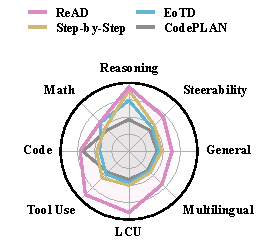
\includegraphics[width=0.45\columnwidth]{figure/rqX_radar_sota_vs_read_150m.pdf}
  \caption{ReAD beats SOTA baselines that are specifically designed for reasoning, code, and math capabilities consistently.}
  % \vspace{-1.2\baselineskip}
  \label{fig:radar}
\end{wrapfigure}

\textbf{ReAD beats SOTA baselines.}
To further validate ReAD against SOTA capability distillation baselines that are specifically designed for certain 
capabilities, we include three representative methods that are commonly used for specializing student models, one per capability: step-by-step distillation~\citep{hsieh2023stepbystep} for reasoning, Equation-of-Thought Distillation (EoTD)~\citep{zhu2024distilling} for math, and CodePLAN~\citep{sun2024enhancing} for code. For a fair comparison under our setting, we adapt each baseline to our LLaMa teacher-student pair and token budget as $150$M, and we distill the student using only the corresponding capability pool. We report the resulting capability profiles on all eight benchmarks using the same evaluation protocol as the main experiments in Figure~\ref{fig:radar}. The results show that these capability-targeted baselines mainly concentrate gains on their target capability and exhibit weaker transfer to other capabilities, producing an imbalanced profile that matches the interaction patterns observed in our empirical study. In contrast, ReAD achieves a consistently stronger and more balanced profile across capabilities, and it is never worse than these baselines on its target capability, while improving substantially on non-target capabilities.


% \subsection{Held-out Downstream Transfer}
% \label{sec:app_xstest}

\textbf{Held-out Downstream Transfer}. To test whether ReAD transfers beyond capability-aligned benchmark tasks, we
evaluate on XSTest using the same requirement identifier and allocation pipeline
without adding a new capability head. Lower safe-refusal and higher
unsafe-refusal scores are better.

\begin{table}[h]
  \centering
  \caption{
  Held-out XSTest evaluation. ``Best baseline'' denotes the best of the six
  SFT/KD baselines for each metric.
  }
  \label{tab:xstest}
  \scriptsize
  \setlength{\tabcolsep}{4pt}
  \renewcommand{\arraystretch}{0.95}

  \begin{tabular}{@{}lcccc@{}}
    \toprule
    \textbf{Method}
      & \textbf{20M safe $\downarrow$}
      & \textbf{20M unsafe $\uparrow$}
      & \textbf{150M safe $\downarrow$}
      & \textbf{150M unsafe $\uparrow$} \\
    \midrule
    Best baseline
      & $15.1\pm0.77$
      & $75.5\pm1.09$
      & $13.1\pm0.69$
      & $79.0\pm0.88$ \\
    \textbf{ReAD}
      & $\mathbf{13.8\pm0.72}$
      & $\mathbf{78.1\pm0.97}$
      & $\mathbf{11.8\pm0.58}$
      & $\mathbf{81.6\pm0.83}$ \\
    \bottomrule
  \end{tabular}
\end{table}

\section{Related Work}
\label{sec:relate}

\textbf{Capability Distillation for Large Language Models.}\label{sec:relate_kd}
Recent work on capability distillation has focused on transferring specific capabilities such as instruction following and context manipulation~\citep{taori2023stanford, chiang2023vicuna, peng2023instruction, xu2023wizardlm}, thinking patterns~\citep{zhang2024knowledgeable, cheng2023adapting}, or text and code generation capability~\citep{zhang2025recommendation, li2023starcoder}. These methods typically steer a teacher LLM via prompts or rationales, generate distillation data or logits, and fine-tune the student on that evidence. However, the majority of methods operate under the assumption that distilling one target capability or domain is sufficient and rarely analyze how that focused training influences broader capability interactions within the student model. To the best of our knowledge, ReAD is the first framework that explicitly accounts for capability interdependence during the distillation.

\section{Broader Impact}
\label{sec:broader_impact}

ReAD aims to make capability distillation more budget-efficient by allocating
limited training tokens across interdependent LLM capabilities. A positive
impact is that smaller student models can become more useful under fixed compute
budgets, potentially reducing deployment cost and improving access to LLM-based
systems in resource-constrained settings. ReAD also explicitly monitors
cross-capability transfer, which can help practitioners diagnose when improving
one capability degrades others.

At the same time, more efficient distillation may lower the cost of producing
specialized models with dual-use capabilities, such as code generation, tool use,
or instruction following. Distilled models may also inherit biases, unsafe
behaviors, privacy risks, or other limitations from teacher models and training
data. In addition, if the capability probes or task requirement vectors are
misaligned with the intended deployment objective, ReAD may optimize benchmark
utility while overlooking safety-, fairness-, or robustness-relevant behaviors.

We therefore view ReAD as a research framework rather than a deployment-ready
safety guarantee. For sensitive applications, practitioners should combine ReAD
with task-specific safety evaluation, robustness and bias audits, data filtering,
red-team testing, and monitoring of off-target capability changes. Any release
or deployment of distilled models should follow the usage restrictions of the
underlying models and include appropriate documentation of intended use,
limitations, and safety evaluations.

\section{Limitation and Future Work}

While ReAD improves budget efficiency by using low-cost capability monitoring and adaptive allocation, it still relies on two practical components that can limit performance. First, the task requirement estimator and the probe suite may be imperfect: if the inferred essential capabilities or probe signals are misaligned with true task utility, ReAD can allocate budget suboptimally. Second, our capability set and data generator are necessarily finite and template-driven, which may not cover all behaviors a real task depends on, especially for highly domain-specific or long-horizon tasks. Future work can address these limitations by learning more robust and transferable task requirement models, designing probe suites with stronger coverage and better calibration to task utility, and expanding capability definitions and data generation beyond templates (e.g., automatic discovery of capability axes and open-ended curriculum generation). Another promising direction is to jointly optimize allocation and student training dynamics (e.g., optimizer schedules and parameter-efficient adapters) under the same budget, and to extend ReAD to settings with distribution shift, multi-task deployment, or continual updates where requirements and transfer patterns evolve over time.

\end{document}
